\documentclass[11pt,a4paper]{article}
\usepackage[utf8]{inputenc}
\usepackage[T1]{fontenc}
\usepackage[brazil]{babel}
\usepackage{lmodern}
\usepackage{amsmath,amssymb,bm}
\usepackage{graphicx,booktabs,float,geometry,url,array,xcolor,caption}
\usepackage[hidelinks]{hyperref}
\geometry{margin=2.2cm}
\captionsetup{font=small}
\emergencystretch=2em
\providecommand{\versao}{sem versão}
% gerado por gera_dados.py; nao edite
\newcommand{\FSzero}{2{,}093}
\newcommand{\patcinqiii}{0{,}832}
\newcommand{\iccinqiii}{39{,}7}
\newcommand{\patcinqi}{0{,}910}
\newcommand{\iccinqi}{23{,}2}
\newcommand{\patcemiii}{1{,}117}
\newcommand{\iccemiii}{--}
\newcommand{\patcemi}{0{,}951}
\newcommand{\iccemi}{5{,}1}
\newcommand{\nRef}{5000}
\newcommand{\falhasRef}{279}
\newcommand{\pfRef}{5{,}58}
\newcommand{\icRefLo}{4{,}98}
\newcommand{\icRefHi}{6{,}25}
\newcommand{\betaRef}{0{,}0768}
\newcommand{\medRef}{1{,}1271}
\newcommand{\fdetRef}{1{,}1239}
\newcommand{\assRef}{0{,}08}
\newcommand{\curtRef}{0{,}05}
\newcommand{\prevMed}{5{,}97}
\newcommand{\prevDet}{6{,}42}
\newcommand{\prevEqSeis}{5{,}73}
\newcommand{\prevLogn}{5{,}89}
\newcommand{\sigmaIiii}{7{,}5}
\newcommand{\decliveiii}{0{,}0102}
\newcommand{\sigmaIi}{3{,}1}
\newcommand{\declivei}{0{,}0247}
\newcommand{\fatorMediana}{1{,}0028}
\newcommand{\nVi}{16}
\newcommand{\dlnMin}{-0{,}300}
\newcommand{\dlnMax}{-0{,}111}
\newcommand{\dlnMed}{-0{,}201}
\newcommand{\dlnSd}{0{,}049}
\newcommand{\pfMaxCemiii}{7{,}5}
\newcommand{\pfMaxCemi}{74{,}2}
\newcommand{\nivelUm}{1{,}196}
\newcommand{\nivelCinco}{1{,}135}
\newcommand{\nivelCinquenta}{1{,}000}
\newcommand{\huBeta}{0{,}0384}
\newcommand{\huM}{0{,}9968}
\newcommand{\betaXL}{0{,}119}
\newcommand{\mXL}{0{,}928}
\newcommand{\ceronBeta}{0{,}238}
\newcommand{\ceronM}{0{,}965}
\newcommand{\rahTangIniCinq}{7{,}3}
\newcommand{\rahTangThrCinq}{50}
\newcommand{\rahSolosProntos}{3}
\newcommand{\mcData}{27/11/2026, 09:13}
\newcommand{\mcFormBetaA}{1{,}60}
\newcommand{\mcFormPfA}{5{,}4}
\newcommand{\mcFragPfA}{3{,}5}
\newcommand{\mcFormBetaB}{0{,}53}
\newcommand{\mcFormPfB}{30{,}0}
\newcommand{\mcFragPfB}{23{,}4}
\newcommand{\mcConf}{0 em 31 na (iii) a 36~mm/h; 0 em 103 na (i) a 30~mm/h; 0 em 120 na (i) a 36~mm/h}
\newcommand{\fragTemiii}{1}
\newcommand{\fragNiii}{2000}
\newcommand{\fragZkiii}{12{,}2}
\newcommand{\fragZkDentroiii}{4 de 7}
\newcommand{\fragZmiii}{-13{,}6}
\newcommand{\fragZmMaxiii}{13{,}6}
\newcommand{\fragZmDentroiii}{3 de 7}
\newcommand{\fragPariii}{27: 9; 30: 5; 31{,}05: 0; 33: 52; 36: 177; 40: 323; 45: 473}
\newcommand{\fragBetaiii}{0{,}077}
\newcommand{\fragMkiii}{1{,}011}
\newcommand{\fragIcaliii}{31{,}05}
\newcommand{\fragTopIiii}{45}
\newcommand{\fragCensMediii}{0{,}998}
\newcommand{\fragCensMedSeiii}{0{,}003}
\newcommand{\fragCensBetaiii}{0{,}108}
\newcommand{\fragCensBetaSeiii}{0{,}003}
\newcommand{\fragPrevMediii}{1{,}024}
\newcommand{\fragPrevMedMedioiii}{0{,}970}
\newcommand{\fragTemi}{1}
\newcommand{\fragNi}{2000}
\newcommand{\fragZki}{9{,}1}
\newcommand{\fragZkDentroi}{2 de 5}
\newcommand{\fragZmi}{-8{,}9}
\newcommand{\fragZmMaxi}{8{,}9}
\newcommand{\fragZmDentroi}{1 de 5}
\newcommand{\fragPari}{18: 43; 20: 0; 22: 139; 24: 295; 36: 398}
\newcommand{\fragBetai}{0{,}085}
\newcommand{\fragMki}{1{,}020}
\newcommand{\fragIcali}{20}
\newcommand{\fragTopIi}{36}
\newcommand{\fragCensMedi}{0{,}914}
\newcommand{\fragCensMedSei}{0{,}005}
\newcommand{\fragCensBetai}{0{,}096}
\newcommand{\fragCensBetaSei}{0{,}004}
\newcommand{\fragPrevMedi}{0{,}948}
\newcommand{\fragPrevMedMedioi}{0{,}905}
\newcommand{\fragCemTem}{1}
\newcommand{\fragCemNiii}{466}
\newcommand{\fragCemBetaiii}{0{,}098}
\newcommand{\fragCemMiii}{1{,}009}
\newcommand{\fragCemBetaCxxiii}{0{,}145}
\newcommand{\fragCemIcaliii}{9}
\newcommand{\fragCemNcaliii}{556}
\newcommand{\fragCemNi}{468}
\newcommand{\fragCemBetai}{0{,}079}
\newcommand{\fragCemMi}{1{,}004}
\newcommand{\fragCemBetaCxxi}{0{,}089}
\newcommand{\fragCemIcali}{3{,}6}
\newcommand{\fragCemNcali}{554}

\newcommand{\Pf}{P_f}
% \input primitivo: funciona dentro de tabular (o \input do LaTeX nao e expansivel)
\makeatletter\newcommand{\tabin}[1]{\@@input #1 }\makeatother
\title{Curva de fragilidade de um talude sob chuva:\\ $P_f(I)$ a partir da sigmoide de Rahardjo et al.\ (2007) e da
primeira passagem\\ \large Formulação, evidências preliminares e a campanha de verificação}
\author{Diogo Cecílio}
\date{25/11/2026 --- versão \versao}
\begin{document}
\maketitle
\begin{abstract}
Rahardjo et al.\ (2007)~\cite{rahardjo2007} mostraram que o fator de segurança mínimo de um talude homogêneo sob chuva segue uma sigmoide
da intensidade, $F(I) = A + B/(1 + e^{-(I-C)/D})$ (a Eq.~6 do artigo). A proposta é levar essa sigmoide para a
probabilidade de ruptura: com propriedades em campos aleatórios, se o FS de cada intensidade for lognormal com mediana
$F(I)$ e dispersão $\beta$, a probabilidade de ruptura é $\Pf(I) = \Phi(-\ln F(I)/\beta)$, uma curva de fragilidade
fechada com cinco constantes: as quatro da sigmoide, de uma varredura determinística barata, e $\beta$, de um único
Monte Carlo de calibração. A ruptura de cada realização é a primeira passagem $T_1$, o instante em que o FS cruza 1: a
simulação pode parar nele, e com chuva constante $\Pf(I, D) = P(T_1(I) \le D)$ dá a probabilidade para todas as
durações de uma vez. Consequência prática: o limiar intensidade--duração de probabilidade $p$ é a curva de nível
$F(I,D) = e^{\beta\,\Phi^{-1}(1-p)}$ do FS determinístico (FS = \nivelCinco{} para 5\,\%). As evidências até agora vêm
do talude de Rahardjo (f50, chuva de 24~h): o FS de 5000 realizações a 31,05~mm/h é lognormal (assimetria de $\ln$ FS
\assRef, $\beta = \betaRef$), e a fórmula com a mediana do MC dá $\prevMed\,\%$ contra $\pfRef\,\%$ do MC direto (IC
95\,\% de $\icRefLo$ a $\icRefHi\,\%$). Com o FS das médias no lugar da mediana a previsão sobe para $\prevDet\,\%$: a
mediana do FS com campo aleatório é $\fatorMediana$ vezes o FS das médias, um efeito pequeno que a esta precisão já
aparece. As sigmoides determinísticas têm $I_c = \iccinqiii$~mm/h com ar passivo e $\iccinqi$~mm/h com ar ativo, uma
quina em $I = k_s$ (o alagamento) e patamares que limitam a $\Pf$ (com ar ativo ela satura em $\approx 88\,\%$; no f100
com 72~h de chuva e ar passivo, em $\approx \pfMaxCemiii\,\%$). Em cinco problemas publicados que recalculamos (Hu et al.\ 2024, Liu et al.\ 2024, Cho 2014, X.\ Liu et al.\ 2025 e
os 26 casos de Vargas Ceron et al.\ 2025), a fórmula prevê a $\Pf$ dentro de um fator $\approx 1{,}5$ entre 0,1 e
20\,\% quando o mecanismo não muda entre os cenários (calibrada num cenário só no caso A de Hu, que varia intensidade e
duração), e fica do lado conservador onde a cauda do FS é mais leve que a lognormal (Ceron); falha quando o $k_s$
aleatório cria um limiar e o FS fica bimodal (a coluna de Cho e X.\ Liu em 24~h). Em dados de oito outros artigos
(Yang et al.\ 2026, Tang et al.\ 2018 e outros) ela reproduz a $\Pf$ contra o CoV da resistência e, no talude de
Rahardjo, $\Pf \approx 50\,\%$ onde o FS determinístico vale 1. A verificação ponto a ponto no fermi (campanha
\texttt{frag}, primeira passagem) responde: no f50 (2000 realizações, completo), com um $\beta$ só, a fórmula acerta
até $I \approx k_s$ e subestima acima dele, onde o $\beta$ cresce (0,077 $\to$ 0,108 com ar passivo); com ar ativo
erra também abaixo da calibração. No f100 (parcial, 466 de 1000 realizações, 72~h) a fórmula fica dentro de $|z|
\le 2{,}6$ em todas as intensidades, e o $\beta$ cresce com a duração.
\end{abstract}
\tableofcontents

\section{A ideia}\label{sec:ideia}
\begin{itemize}
  \item \textbf{O ponto de partida.} No estudo paramétrico de Rahardjo et al.\ (2007)~\cite{rahardjo2007}, o FS mínimo de um talude
    homogêneo cai com a intensidade da chuva $I$ segundo uma sigmoide (Fig.~6 e Eq.~6 do artigo): constante nas chuvas
    fracas, caindo depois da intensidade inicial $I_{ini}$ e parando num patamar inferior a partir da intensidade-limite
    $I_{thr}$. É um resultado determinístico: o talude rompe ou não.
  \item \textbf{A pergunta.} Com a variabilidade espacial das propriedades (campos aleatórios de $c'$, $\varphi'$ e
    $k_s$), qual é a probabilidade de ruptura em função da chuva, $\Pf(I)$? É possível escrevê-la com as constantes da
    sigmoide, e com poucas simulações?
  \item \textbf{A proposta.} $\Pf(I) = \Phi(-\ln F(I)/\beta)$: a sigmoide determinística dá a mediana do FS, e uma
    única dispersão $\beta$ espalha o FS das realizações em torno dela (Seção~\ref{sec:form}). A ruptura é a primeira
    passagem $T_1$ (o FS cruza 1), que também dá a duração (Seção~\ref{sec:t1}).
  \item \textbf{O produto.} Uma fórmula fechada $\Pf(I)$, e $\Pf(I, D)$, para um talude e um material, com cinco
    constantes, e os limiares intensidade--duração de probabilidade dada (Seção~\ref{sec:limiares}).
\end{itemize}

\section{Formulação}\label{sec:form}

\subsection{A sigmoide determinística e a intensidade crítica}
Seja $F(I)$ o FS do talude com as propriedades médias no fim de uma chuva de intensidade constante $I$ e duração $D$
(no f50 com $D = 24$~h, o FS mínimo da história). Rahardjo et al.\ (2007) ajustam
\begin{equation}
F(I) = A + \frac{B}{1 + e^{-(I - C)/D_s}},\label{eq:sig}
\end{equation}
com $A$ o patamar das chuvas fracas, $A + B$ ($B < 0$) o patamar das fortes, $C$ o centro e $D_s$ a largura
(escrevemos $D_s$ para não confundir com a duração). O talude rompe com as propriedades médias a partir da
intensidade crítica
\begin{equation}
F(I_c) = 1 \quad\Longleftrightarrow\quad I_c = C - D_s \ln\!\left(\frac{B}{1 - A} - 1\right),\qquad A + B < 1 < A.
\label{eq:ic}
\end{equation}
Se o patamar inferior $A + B$ fica acima de 1, o talude médio não rompe com nenhuma intensidade daquela duração.
Fisicamente $A$ é o FS sem chuva (o FS inicial, \FSzero{} no talude de Rahardjo), o que fixa uma constante.

\subsection{Do FS aleatório à probabilidade: a curva de fragilidade}
Com campos aleatórios $\bm\xi$, o FS da realização, $\mathrm{FS}(I;\bm\xi)$, é uma variável aleatória. Duas hipóteses:
\begin{itemize}
  \item \textbf{H1 (lognormal):} para cada $I$, $\ln \mathrm{FS}(I;\bm\xi) \sim \mathcal N(\ln \tilde F(I), \beta^2)$.
  \item \textbf{H2 (parâmetros):} a mediana segue o determinístico, $\tilde F(I) = m\,F(I)$ com $m$ constante (perto de
    1), e $\beta$ não depende de $I$.
\end{itemize}
Então
\begin{equation}
\boxed{\;\Pf(I) = P[\mathrm{FS}(I;\bm\xi) < 1] = \Phi\!\left(-\frac{\ln m F(I)}{\beta}\right)\;}\label{eq:frag}
\end{equation}
é a curva de fragilidade do talude. Propriedades, com $m = 1$:
\begin{itemize}
  \item \textbf{Centro:} $\Pf(I_c) = 50\,\%$: a intensidade crítica determinística é a mediana da intensidade de
    ruptura.
  \item \textbf{Largura:} perto de $I_c$, $\Pf(I) \approx \Phi\big((I - I_c)/\sigma_I\big)$ com
    $\sigma_I = \beta / |{\rm d}\ln F/{\rm d}I|_{I_c}$. A incerteza das propriedades ``borra'' o degrau determinístico
    em $I_c$ numa rampa de largura $\sigma_I$: quanto mais íngreme a sigmoide em $I_c$, mais estreita a rampa.
  \item \textbf{Patamares:} $\Pf(0) = \Phi(-\ln A/\beta) \approx 0$ e $\Pf(\infty) = \Phi(-\ln(A+B)/\beta)$. Se o
    patamar inferior do FS fica perto de 1, a $\Pf$ satura abaixo de 100\,\% (ou acima de 0): a chuva mais forte não
    rompe mais realizações.
  \item \textbf{Constantes:} $A, B, C, D_s$ (uma varredura determinística, $\approx 3$~min de PC) e $\beta$ (um MC numa
    intensidade); $m$, se necessário, do mesmo MC (a razão entre a mediana do MC e $F$).
\end{itemize}
A forma (\ref{eq:frag}) é a curva de fragilidade lognormal da engenharia sísmica, com a intensidade da chuva no lugar
da medida de intensidade do sismo; a diferença é que aqui a mediana não é um parâmetro livre, mas a sigmoide
determinística do próprio talude.

\subsection{A primeira passagem e a duração}\label{sec:t1}
A ruptura de uma realização é o primeiro instante em que o FS cruza 1,
\begin{equation}
T_1(I;\bm\xi) = \inf\{t \ge 0 : \mathrm{FS}(t; I, \bm\xi) < 1\},
\end{equation}
e não o FS mínimo da história: depois de $T_1$ o cálculo usa a geometria intacta e as pressões de um talude que já
rompeu, sem sentido físico; a simulação pode parar em $T_1$. Com chuva de intensidade constante, a realização que rompe
em $T_1$ rompe em qualquer chuva da mesma intensidade com duração $D \ge T_1$, logo
\begin{equation}
\Pf(I, D) = P[T_1(I) \le D]\label{eq:pfid}
\end{equation}
para todas as durações até a simulada, a partir de \emph{uma} simulação por intensidade. Se, além disso, o FS só cai
durante a chuva (o que vale nos casos calculados), $\{T_1 \le D\} = \{\mathrm{FS}(D) < 1\}$ e a fórmula
(\ref{eq:frag}) se estende para $\Pf(I, D) = \Phi(-\ln m F(I, D)/\beta)$, com $F(I, D)$ o FS das médias no fim de uma
chuva $(I, D)$.

\textbf{O algoritmo} (opção \texttt{crpc=} do \texttt{SlopeRainMonteCarlo}, a curva crítica de Liu e Wang (2023)~\cite{liuwang2023}
estendida às variantes acopladas): para cada realização, as intensidades em ordem decrescente; em cada uma, chuva
constante até $D_{\max}$, o FS em 6, 12, 24, 48, 96~h e $D_{\max}$, e bissecção nas horas guardadas entre o último
instante com FS $\ge 1$ e o primeiro com FS $< 1$; $T_1$ por interpolação linear. Quem não rompe numa intensidade não
roda as menores ($T_1$ cai com $I$: monotonia). A curva de fragilidade empírica é a distribuição de $T_1$ (ou da
intensidade crítica de cada realização), com os mesmos campos em todas as intensidades.

\subsection{Limiares intensidade--duração de probabilidade dada}\label{sec:limiares}
De $\Pf(I, D) = p$ vem
\begin{equation}
F(I, D) = \frac{1}{m}\,e^{\beta\,\Phi^{-1}(1-p)}:\label{eq:limiar}
\end{equation}
o limiar intensidade--duração de probabilidade $p$ é uma \emph{curva de nível do FS determinístico}. Com $\beta =
\betaRef$ e $m = 1$: $\Pf = 1\,\%$ em FS = \nivelUm, $5\,\%$ em FS = \nivelCinco{} e $50\,\%$ em FS = \nivelCinquenta. O
mapa determinístico $F(I, D)$, barato, vira o mapa de probabilidade com uma constante.

\section{Evidências preliminares}\label{sec:evid}
Os dados abaixo já existem (25/11/2026; variante (iii): desacoplado, esqueleto rígido, ar passivo, as hipóteses do
artigo; variante (i): acoplado, esqueleto elástico, ar ativo). Talude de Rahardjo ($45^\circ$, $H_s = 10$~m,
$H_w = 5$~m), campos de Karhunen--Loève de $c'$, $\varphi'$ e $k_s$ com as estatísticas da Tabela~2 de Vargas Ceron et
al.\ (2025)~\cite{ceron2025} (CoV 0,3; 0,1; 0,6; distâncias de autocorrelação de 20 e 2~m), FS pelo SRM.

\subsection{As sigmoides determinísticas}
\begin{figure}[H]\centering
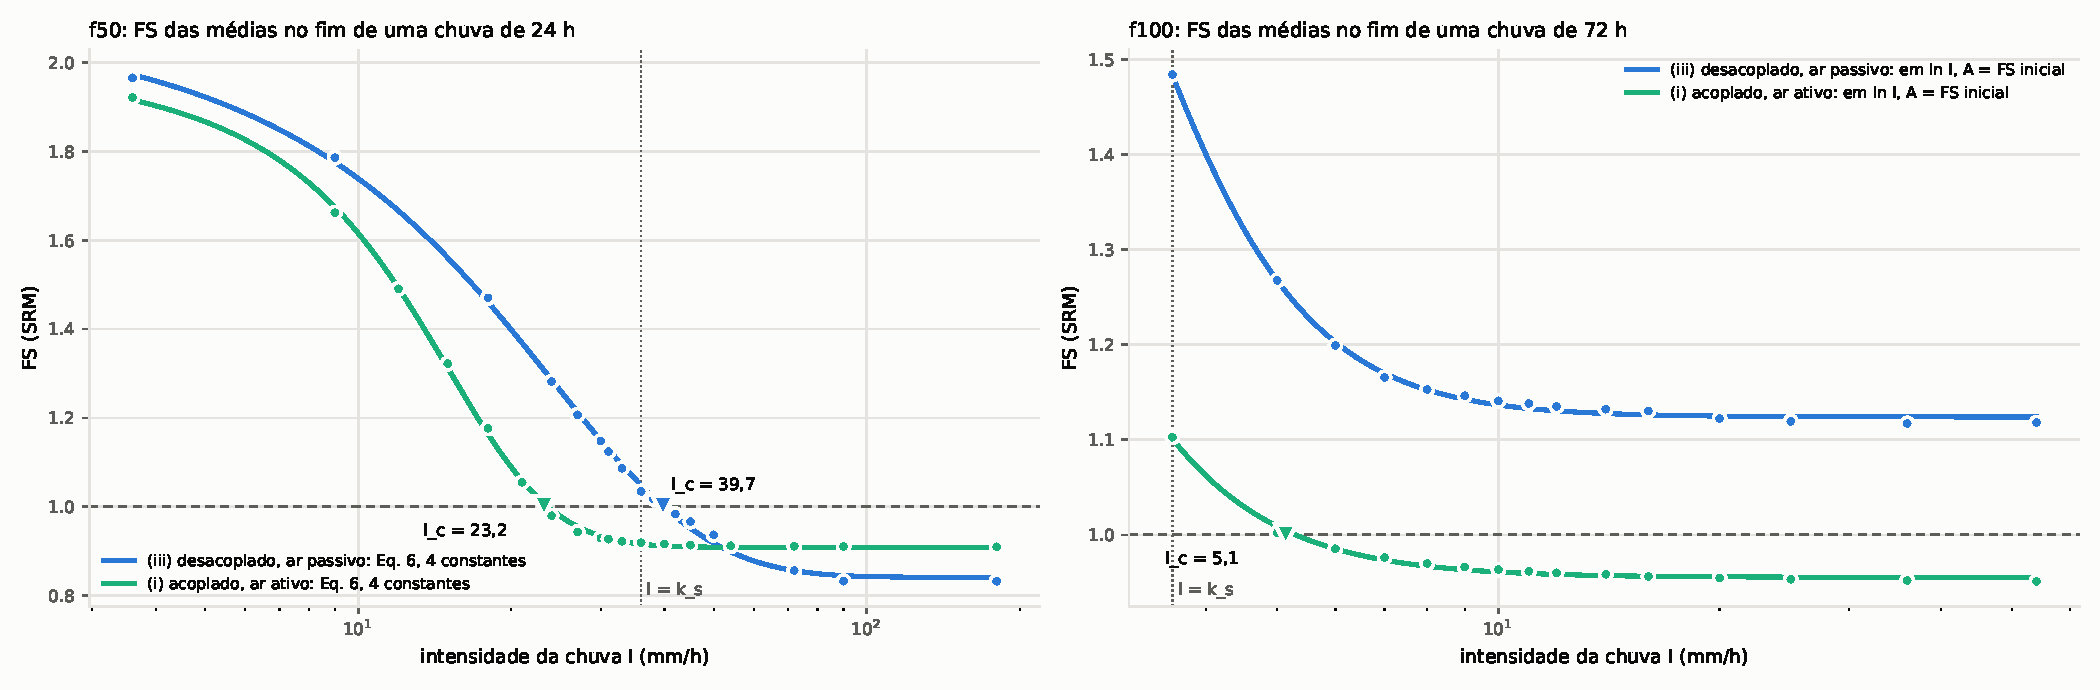
\includegraphics[width=\textwidth]{figs/sigmoides.pdf}
\caption{FS das médias no fim da chuva contra $I$: f50 com 24~h (18 intensidades) e f100 com 72~h (15), variantes
(iii) e (i); linhas: a forma adotada da sigmoide (Tabela~\ref{tab:sig}); triângulos: $I_c$.}\label{fig:sig}
\end{figure}

\begin{table}[H]\centering\scriptsize\setlength{\tabcolsep}{3.5pt}
\caption{As três formas da sigmoide ajustadas: a Eq.~6 com as 4 constantes livres, a Eq.~6 com $A$ = FS inicial e a
mesma sigmoide em $\ln I$ com $A$ = FS inicial; $\star$ a forma adotada (o menor resíduo perto de FS = 1, entre 0,9 e
1,25). Resíduos em FS.}\label{tab:sig}
\resizebox{\textwidth}{!}{%
\begin{tabular}{llccccccc}
\toprule
caso & forma & $A$ & $B$ & $C$ & $D_s$ & $A + B$ & resíduo rms & resíduo máx. perto de 1\\
\midrule
\tabin{tab/sigmoides.tex}
\bottomrule
\end{tabular}}
\end{table}

\begin{itemize}
  \item \textbf{Intensidade crítica:} no f50, $I_c = \iccinqiii$~mm/h com ar passivo e $\iccinqi$~mm/h com ar ativo;
    no f100 com 72~h, o talude médio não rompe com ar passivo (o FS para num patamar de \patcemiii{} acima de
    $\approx 10$~mm/h $\approx 3k_s$) e rompe a partir de $\iccemi$~mm/h com ar ativo.
  \item \textbf{A quina em $I = k_s$} (f50, iii): abaixo de $k_s$ toda a chuva entra e o FS cai $\approx 0{,}018$ por
    mm/h; acima a superfície alaga, a infiltração fica limitada e o FS cai \decliveiii{} em $\ln$ por mm/h perto de
    $I_c$. Nenhuma das três formas suaves a reproduz bem: a Eq.~6 com 4 constantes é a que menos erra perto de FS = 1
    (resíduo máximo 0,019), à custa de um $A$ sem sentido físico (2,78 contra o FS inicial \FSzero).
  \item \textbf{Os patamares:} \patcinqiii{} (f50, iii), \patcinqi{} (f50, i), \patcemiii{} (f100, iii, 72~h) e
    \patcemi{} (f100, i, 72~h). Com ar ativo o patamar do f50 é mais alto que com ar passivo, mas é atingido muito
    antes ($\approx 30$~mm/h contra $\approx 90$).
  \item \textbf{A forma depende do caso:} no f100 a Eq.~6 em $I$ degenera (os dados não mostram o patamar superior), e
    a forma em $\ln I$ com $A$ = FS inicial ajusta com resíduo de 0,003--0,004.
\end{itemize}

\subsection{As Figs.~6 e 7 de Rahardjo et al.\ (2007) para os três solos}\label{sec:rahardjo67}
\providecommand{\rahTangIniCinq}{--}\providecommand{\rahTangThrCinq}{--}
Rahardjo et al.\ (2007)~\cite{rahardjo2007} varreram a intensidade de uma chuva de 24~h nos três solos (f10, f50 e f100,
com $k_s$ = 360, 36 e 3,6~mm/h) e ajustaram a Eq.~6 ao $F_{s(min)}$ de cada um (a Fig.~7 do artigo traz as constantes).
No gráfico semilog, a tangente no ponto mais íngreme da sigmoide corta o patamar de cima em $I_{r(ini)}$, onde o FS
começa a cair, e o de baixo em $I_{r(thr)}$, a partir de onde chover mais forte não baixa mais o FS. A
Fig.~\ref{fig:rah6} refaz a Fig.~6 do artigo com as nossas contas, a Fig.~\ref{fig:rah7} refaz a Fig.~7, e a
Tab.~\ref{tab:rahconst} compara as constantes. Entram as variantes (iii), que é o modelo do artigo (percolação
desacoplada, ar passivo), e (i).
\begin{itemize}
  \item \textbf{O $F_{s(min)}$ é o FS das médias no fim da chuva de 24~h.} Nos três solos o mínimo cai no fim da chuva;
    no f100 com 72~h de chuva, o mínimo depois dela fica 0,008 abaixo, dentro da resolução do SRM.
  \item \textbf{O ajuste usa a forma do artigo:} $I$ linear, com $D < 0$, e $A$ é o patamar de baixo. As tangentes são
    calculadas, enquanto o artigo as traçou à mão. Aplicada às constantes do artigo, a nossa construção dá
    $I_{r(ini)} = \rahTangIniCinq$ e $I_{r(thr)} = \rahTangThrCinq$~mm/h no f50 (o artigo: 8,5 e 51).
  \item \textbf{As varreduras:} o f50 tem 18 intensidades de 3,6 a 180~mm/h; o f100 tem 15, de 3,6 a 54~mm/h (o FS de
    24~h das chuvas de 72~h). O f10 inteiro e os patamares que faltavam (0,36 a 2,7~mm/h no f50 e no f100; 360~mm/h no
    f50; 90~mm/h no f100) estão na fila do PC (\texttt{runs/rahardjo\_3solos}).
\end{itemize}

\begin{figure}[H]\centering
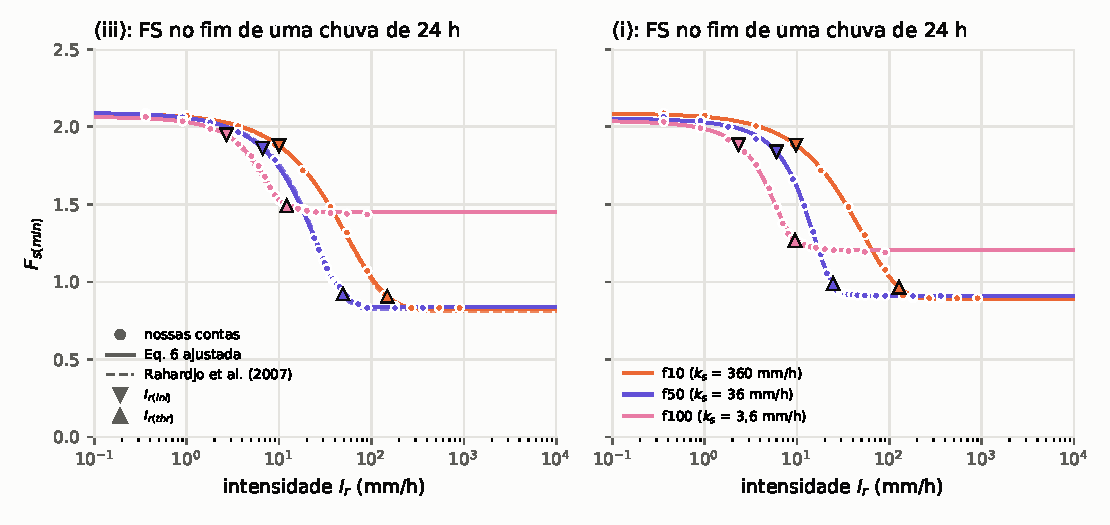
\includegraphics[width=\textwidth]{figs/rahardjo_fig6.pdf}
\caption{A Fig.~6 de Rahardjo et al.\ (2007) com as nossas contas: o FS das médias no fim de uma chuva de 24~h contra a
intensidade, nos três solos. Pontos: as nossas análises; linha cheia: a Eq.~6 ajustada a eles; tracejada: a Eq.~6 com as
constantes do artigo; triângulos: $I_{r(ini)}$ ($\triangledown$) e $I_{r(thr)}$ ($\vartriangle$).}\label{fig:rah6}
\end{figure}

\begin{table}[H]\centering\small
\caption{As constantes da Eq.~6 na forma do artigo, $F_{s(min)} = A + B/(1 + e^{-(I_r - C)/D})$ com $I_r$ em mm/h.
``idem, nossas tangentes'': a nossa construção das tangentes aplicada às constantes do artigo. FS(0): o FS inicial, sem
chuva. $I_c$: a intensidade em que a Eq.~6 vale 1 (mm/h).}\label{tab:rahconst}
\resizebox{\textwidth}{!}{\begin{tabular}{lrlrrrrrrlll}
\toprule
solo & $k_s$ (mm/h) & fonte & $A$ & $B$ & $C$ & $D$ & $r^2$ & FS(0) & $I_{r(ini)}$ ($\times k_s$) & $I_{r(thr)}$ ($\times k_s$) & $I_c$\\
\midrule
f10 & 360 & Rahardjo et al. & 0{,}81 & 13{,}54 & -118{,}00 & -52{,}00 & 0{,}999 & -- & 11{,}0 (0{,}03) & 140 (0{,}39) & 103{,}1\\
 & & idem, nossas tangentes & & & & & & & 10{,}4 (0{,}03) & 146 (0{,}41) & --\\
 & & nosso, (iii) & 0{,}82 & 41{,}86 & -187{,}07 & -53{,}90 & 0{,}999 & 2{,}093 & 10{,}0 (0{,}03) & 148 (0{,}41) & 107{,}7\\
 & & nosso, (i) & 0{,}89 & 6{,}36 & -63{,}43 & -43{,}50 & 0{,}999 & 2{,}093 & 9{,}8 (0{,}03) & 127 (0{,}35) & 110{,}9\\
\addlinespace
f50 & 36 & Rahardjo et al. & 0{,}82 & 1{,}83 & 10{,}70 & -13{,}13 & 0{,}997 & -- & 8{,}5 (0{,}24) & 51 (1{,}42) & 39{,}8\\
 & & idem, nossas tangentes & & & & & & & 7{,}3 (0{,}20) & 50 (1{,}40) & --\\
 & & nosso, (iii) & 0{,}84 & 1{,}91 & 8{,}41 & -13{,}15 & 1{,}000 & 2{,}093 & 6{,}6 (0{,}18) & 49 (1{,}36) & 39{,}8\\
 & & nosso, (i) & 0{,}91 & 1{,}28 & 11{,}01 & -5{,}08 & 0{,}999 & 2{,}093 & 6{,}0 (0{,}17) & 25 (0{,}68) & 23{,}9\\
\addlinespace
f100 & 3{,}6 & Rahardjo et al. & 1{,}45 & 0{,}70 & 4{,}75 & -2{,}35 & 0{,}998 & -- & 2{,}8 (0{,}78) & 11 (3{,}06) & --\\
 & & idem, nossas tangentes & & & & & & & 2{,}6 (0{,}71) & 11 (3{,}08) & --\\
 & & nosso, (iii) & 1{,}45 & 0{,}71 & 4{,}98 & -2{,}61 & 0{,}998 & 2{,}093 & 2{,}7 (0{,}75) & 12 (3{,}35) & --\\
 & & nosso, (i) & 1{,}21 & 0{,}93 & 4{,}26 & -1{,}97 & 0{,}999 & 2{,}093 & 2{,}3 (0{,}64) & 10 (2{,}64) & --\\
\bottomrule
\end{tabular}
}
\end{table}

\begin{figure}[H]\centering
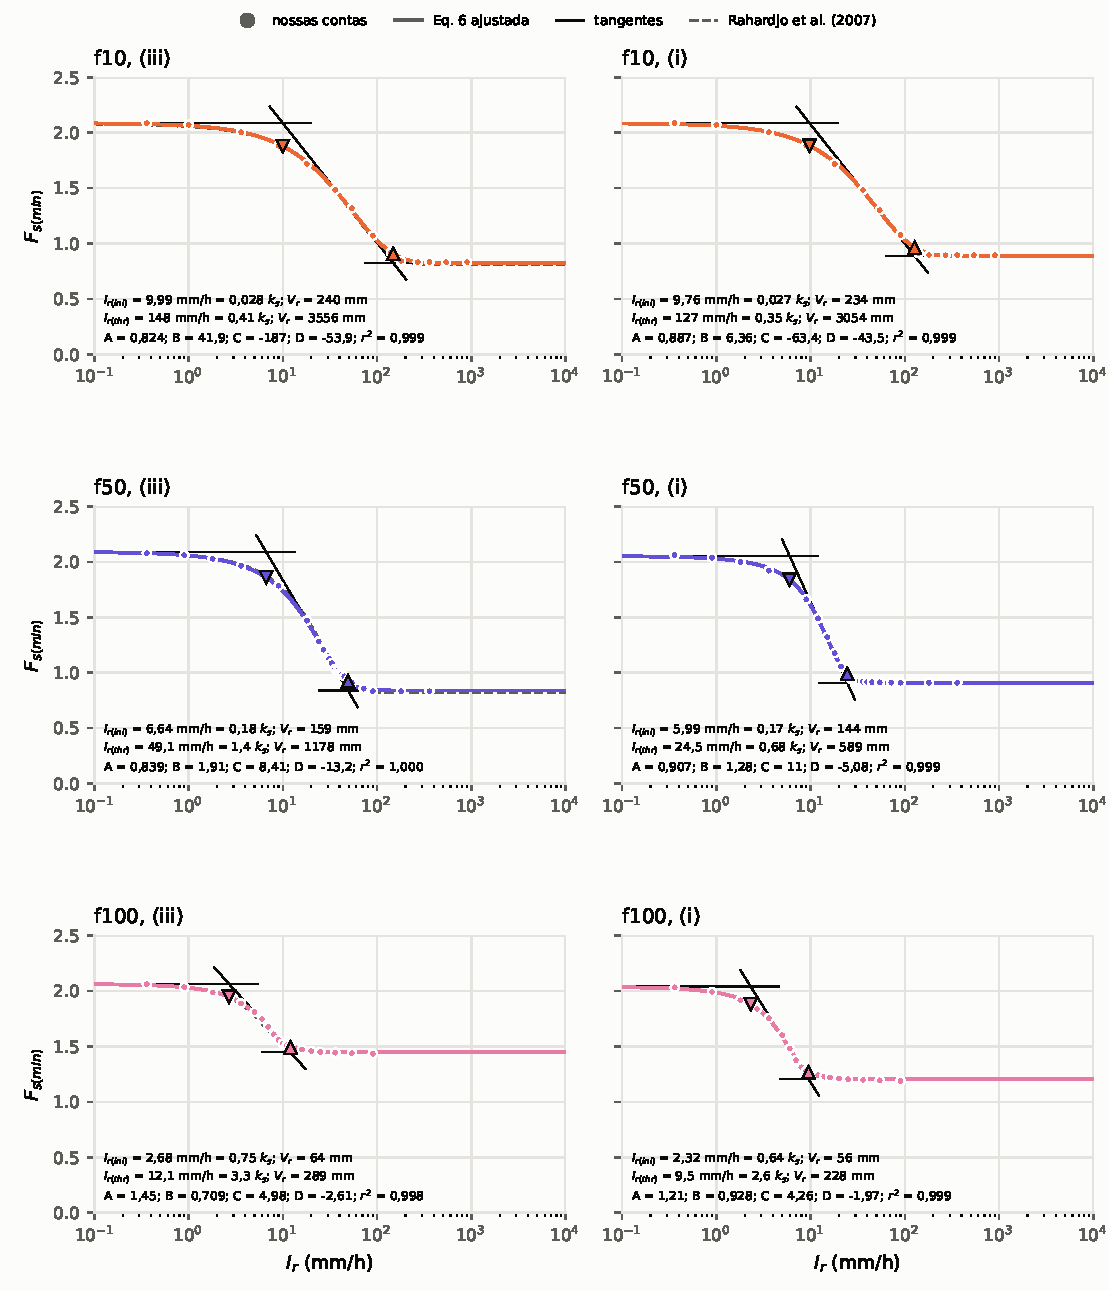
\includegraphics[width=\textwidth]{figs/rahardjo_fig7.pdf}
\caption{A Fig.~7 de Rahardjo et al.\ (2007) com as nossas contas: um painel por solo (linhas) e variante (colunas),
com a Eq.~6 ajustada, as constantes, o $r^2$ e as tangentes; $I_{r(ini)}$ e $I_{r(thr)}$ também como múltiplos de $k_s$ e
como o volume de chuva $V_r = 24\,I_r$. Tracejada: a Eq.~6 com as constantes do artigo, só na (iii).}\label{fig:rah7}
\end{figure}

\subsection{A referência: o FS de 5000 realizações é lognormal}
\begin{figure}[H]\centering
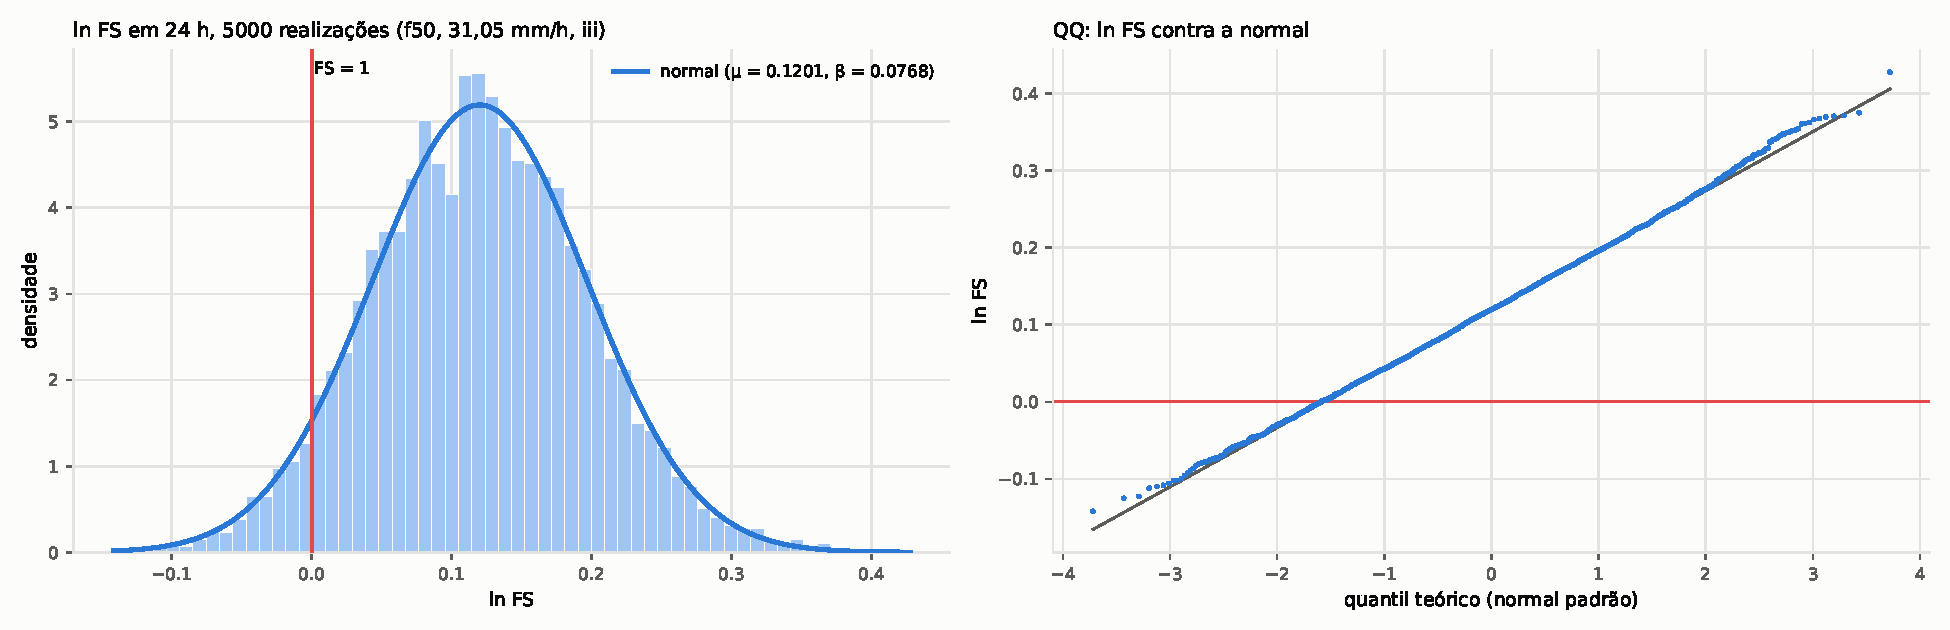
\includegraphics[width=\textwidth]{figs/referencia.pdf}
\caption{f50, variante (iii), 31,05~mm/h por 24~h, \nRef{} realizações (MC direto da campanha \texttt{chuva2}): o
histograma de $\ln$ FS em 24~h com a normal ajustada e o gráfico QQ.}\label{fig:ref}
\end{figure}

\begin{table}[H]\centering\small
\caption{A $\Pf$ prevista pela fórmula (\ref{eq:frag}) na referência, contra o MC direto: $\Pf = \pfRef\,\%$
(\falhasRef{} falhas em \nRef; IC 95\,\% de \icRefLo{} a $\icRefHi\,\%$). $z$: a diferença em erros padrão do MC.}
\label{tab:ref}
\begin{tabular}{lcc}
\toprule
mediana usada & $\Pf$ prevista & $z$\\
\midrule
\tabin{tab/ref.tex}
\bottomrule
\end{tabular}
\end{table}

\begin{itemize}
  \item \textbf{H1 se sustenta na referência:} $\ln$ FS tem assimetria \assRef{} e curtose em excesso \curtRef; o QQ é
    reto também na cauda de baixo, que é a que conta. A lognormal ajustada dá $\prevLogn\,\%$ ($z < 1$).
  \item \textbf{$\beta = \betaRef$:} a dispersão de $\ln$ FS com $c'$, $\varphi'$ e $k_s$ aleatórios. Ela é pequena: um
    erro de 0,01 no FS mediano desloca a $\Pf$ prevista em $\approx 0{,}13\,\beta$, ou cerca de 1,5 ponto a 6\,\%.
  \item \textbf{A mediana do FS não é o FS das médias:} \medRef{} contra \fdetRef{} (fator $m = \fatorMediana$). Com a
    mediana do MC a fórmula acerta ($\prevMed\,\%$, $z \approx 1$); com o FS das médias erra por $z \approx 2{,}6$
    ($\prevDet\,\%$). O efeito é pequeno (0,3\,\% no FS) e só aparece com 5000 realizações; se $m$ for constante, ele
    entra como sexta constante, do mesmo MC de calibração. A sigmoide adotada dá $\prevEqSeis\,\%$, mas por compensação
    (o resíduo do ajuste nesse ponto, $-0{,}005$, tem o mesmo tamanho e o sinal contrário de $m$).
\end{itemize}

\subsection{A variante com ar ativo em campo aleatório}
Em \nVi{} realizações da referência (8 das de menor FS, 4 perto de FS = 1 e 4 sorteadas; amostra dirigida, não
aleatória), a variante (i) baixa $\ln$ FS em 24~h de \dlnMax{} a \dlnMin{} (média \dlnMed, desvio \dlnSd) em relação à
(iii). O deslocamento varia de realização para realização (depende do campo de $k_s$, que controla o ar aprisionado):
somado à dispersão da (iii), deve dar $\beta$ maior com ar ativo (da ordem de $\sqrt{0{,}077^2 + 0{,}05^2} \approx
0{,}09$ se forem independentes). O MC de calibração da campanha mede.

\subsection{A primeira passagem}
\begin{table}[H]\centering\small
\caption{Determinístico (as médias), os 3 solos com chuvas de 24~h (relatório \texttt{det\_3solos}): o FS mínimo e
$T_1$ (h) nas três variantes; -- : não rompe.}\label{tab:t1det}
\begin{tabular}{ll cc cc cc}
\toprule
 & & \multicolumn{2}{c}{(iii)} & \multicolumn{2}{c}{(ii)} & \multicolumn{2}{c}{(i)}\\
\cmidrule(lr){3-4}\cmidrule(lr){5-6}\cmidrule(lr){7-8}
solo & $I$ (mm/h) & FS mín. & $T_1$ & FS mín. & $T_1$ & FS mín. & $T_1$\\
\midrule
\tabin{tab/t1_det.tex}
\bottomrule
\end{tabular}
\end{table}

\begin{table}[H]\centering\small
\caption{O algoritmo da primeira passagem em realizações da referência (f50, 24~h): $T_1$ (h) por intensidade
(mm/h). FS 31,05: o FS em 24~h da realização no MC direto da referência.}\label{tab:crpc}
\begin{tabular}{lcc p{10.5cm}}
\toprule
realização & var. & FS 31,05 & $T_1$ por intensidade\\
\midrule
\tabin{tab/crpc_teste.tex}
\bottomrule
\end{tabular}
\end{table}

\begin{itemize}
  \item \textbf{$T_1$ e FS mínimo contam histórias diferentes} (Tabela~\ref{tab:t1det}): com ar ativo o FS mínimo do
    f10 com 180~mm/h e do f50 com 90~mm/h é \emph{maior} que com ar passivo, mas a ruptura vem 5 e 8~h antes. Para a
    probabilidade, o evento é $T_1 \le D$.
  \item \textbf{O algoritmo funciona nas duas variantes} (Tabela~\ref{tab:crpc}): $T_1$ cresce quando $I$ cai, como a
    monotonia pede; a realização que não rompe com 45~mm/h não roda as intensidades menores; e o $T_1$ a 31,05~mm/h
    concorda com o FS do MC direto na mesma realização (rompe antes de 24~h quando o FS em 24~h é menor que 1).
\end{itemize}

\subsection{Casos calculados em comum com outros artigos}\label{sec:testes}
Cinco problemas publicados foram recalculados por nós (os mesmos taludes, propriedades e chuvas, com o MEF do NeoPZ, ou
em Python no caso de X.\ Liu et al.\ \cite{xliu2025}). As Tabelas~\ref{tab:hu} a \ref{tab:cer} põem lado a lado a
$\Pf$ do artigo, a nossa (MC direto e line sampling, com o CoV da estimativa) e a da fórmula (\ref{eq:frag}). Nas
fórmulas, a mediana e $\beta$ vêm de um MC de calibração (dito em cada tabela); ``lida'' indica valor tirado de figura.
CoV do MC: $\sqrt{(1 - \Pf)/(N\Pf)}$.

\begin{table}[H]\centering\scriptsize\setlength{\tabcolsep}{3pt}
\caption{Hu et al.\ \cite{hu2024}, caso A (talude de 10~m a $45^\circ$, $k_s$ fixo, $c'$ e $\varphi'$ em campos com
$r = -0{,}5$): $\Pf$ (\%) por cenário de chuva. Artigo: PDET com 180 realizações. Fórmula: $\beta = \huBeta$ e $m = \huM$
calibrados no cenário de 30~mm/h por 24~h; $z$: fórmula contra o LS.}\label{tab:hu}
\resizebox{\textwidth}{!}{%
\begin{tabular}{cc c c ccc cc cc}
\toprule
 & & & artigo & \multicolumn{3}{c}{nosso MC} & \multicolumn{2}{c}{nosso LS} & \multicolumn{2}{c}{fórmula}\\
\cmidrule(lr){5-7}\cmidrule(lr){8-9}\cmidrule(lr){10-11}
$I$ (mm/h) & $D$ (h) & $F$ & $\Pf$ & falhas/$N$ & $\Pf$ & CoV (\%) & $\Pf$ & CoV (\%) & $\Pf$ & $z$\\
\midrule
\tabin{tab/comum_hu.tex}
\bottomrule
\end{tabular}}
\end{table}

\begin{table}[H]\centering\scriptsize\setlength{\tabcolsep}{3pt}
\caption{Liu et al.\ \cite{liu2024}, caso B, e o mesmo talude em Yang et al.\ \cite{yang2026}: $\Pf$ (\%). $F$: o
nosso FS das médias (SRM; Bishop dá 1,525--1,527 nos dois artigos). Artigo: Tabela~4 (lognormal ajustada a 2000
realizações) e Tabela~2 (hipercubo latino, cenário 3); as duas não fecham entre si. Fórmula: com a mediana e o $\beta$
do nosso MC, e com $F$ no lugar da mediana.}\label{tab:liuB}
\resizebox{\textwidth}{!}{%
\begin{tabular}{l c ccc c cc cc}
\toprule
 & & \multicolumn{2}{c}{artigo} & Yang & nosso MC & \multicolumn{2}{c}{nosso LS} & \multicolumn{2}{c}{fórmula}\\
\cmidrule(lr){3-4}\cmidrule(lr){7-8}\cmidrule(lr){9-10}
cenário & $F$ & Tab.~4 & Tab.~2 & (2026) & falhas/$N$ (lim.\ sup.\ 95\,\%) & $\Pf$ & CoV (\%) & mediana & $F$\\
\midrule
\tabin{tab/comum_liu.tex}
\bottomrule
\end{tabular}}
\end{table}

\begin{table}[H]\centering\scriptsize\setlength{\tabcolsep}{3pt}
\caption{Cho \cite{cho2014} (coluna de talude infinito, $k_s$ em campo, 15 casos de CoV e $l_v$): $\Pf$ (\%) em 18 e 24~h,
o artigo e o nosso MC do NeoPZ (\texttt{SlopeRainColumn}; o MC em Python dá 1,45 e 36,87\,\% no caso base com 55\,000
realizações). Fórmula em 24~h: o FS das médias (0,367 em todos) e o $\beta$ do próprio MC.}\label{tab:chocomum}
\begin{tabular}{lc ccc ccc c}
\toprule
 & & \multicolumn{3}{c}{18~h} & \multicolumn{3}{c}{24~h} & fórmula\\
\cmidrule(lr){3-5}\cmidrule(lr){6-8}
caso & $N$ & artigo & nosso & CoV (\%) & artigo & nosso & CoV (\%) & 24~h\\
\midrule
\tabin{tab/comum_cho.tex}
\bottomrule
\end{tabular}
\end{table}

\begin{table}[H]\centering\small
\caption{X.\ Liu et al.\ \cite{xliu2025}, caso 1 (talude infinito, 3~cm/h; $k_s$, $c'$, $\varphi'$ a posteriori e viés de
modelo): $\Pf$ (\%) no tempo. $F$: rótulos da Fig.~12 (lidos). Nosso: reprodução em Python (0~h com $10^4$; 12 e 24~h,
MC de 300). Fórmula: $\beta = \betaXL$ e $m = \mXL$ ajustados de 0 a 18~h (4 pontos, 2 parâmetros); 24~h é previsão.}
\label{tab:xliu}
\begin{tabular}{cc ccc}
\toprule
$t$ (h) & $F$ & artigo & nosso & fórmula\\
\midrule
\tabin{tab/comum_xliu.tex}
\bottomrule
\end{tabular}
\end{table}

\begin{table}[H]\centering\scriptsize\setlength{\tabcolsep}{2.5pt}
\caption{Vargas Ceron et al.\ \cite{ceron2025} (rebaixamento; $\Gamma$ pelo GIM; os 26 casos das Seções 6.1 a 6.5):
$\Pf$ (\%) do artigo (com o CoV da estimativa), do nosso LS e do nosso MC pareado de 500. Fórmula A: a lognormal com a
mediana e o $\beta$ do MC do próprio caso (H1). Fórmula B: $\beta = \ceronBeta$ e $m = \ceronM$ da referência, nas
famílias que mudam o $\Gamma$ determinístico ($\alpha$ e $h_w/H$, os análogos da intensidade da chuva; H2). $z$:
contra o LS.}\label{tab:cer}
\resizebox{\textwidth}{!}{%
\begin{tabular}{lc c cc cc c c cc cc}
\toprule
 & & & \multicolumn{2}{c}{artigo} & \multicolumn{2}{c}{nosso LS} & MC & & \multicolumn{2}{c}{fórmula A} &
\multicolumn{2}{c}{fórmula B}\\
\cmidrule(lr){4-5}\cmidrule(lr){6-7}\cmidrule(lr){10-11}\cmidrule(lr){12-13}
caso & seção & $\Gamma_{det}$ & $\Pf$ & CoV & $\Pf$ & CoV & $\Pf$ & $\beta$ & $\Pf$ & $z$ & $\Pf$ & $z$\\
\midrule
\tabin{tab/comum_ceron.tex}
\bottomrule
\end{tabular}}
\end{table}

\paragraph{O que os casos em comum mostram.}
\begin{itemize}
  \item \textbf{Hu, caso A (intensidade e duração).} $\beta$ (0,038--0,042) e $m$ (0,995--0,997) quase não mudam entre os
    seis cenários, e $\ln$ FS é simétrico. Calibrada num cenário, a fórmula acerta o de 20~mm/h por 36~h (0,25 contra
    0,27\,\% do LS, $z = -1{,}4$); no de 40~mm/h por 12~h fica 1,5 vez acima do LS (0,11 contra 0,072\,\%, $z = +4{,}6$),
    mas dentro do IC do MC; com 50~mm/h, $1 - \Pf$ fica 2 vezes acima. Nas caudas extremas ($< 10^{-6}$) não vale. A
    $\Pf$ do artigo não se reproduz (22\,\% contra 7\,\% a 30~mm/h por 24~h): o desvio do FS de Hu passa do limite
    homogêneo (relatório \texttt{hu2024}).
  \item \textbf{Liu, caso B (a cauda).} Com a mediana do MC a lognormal fica dentro do CoV do LS ($6{,}4 \cdot 10^{-6}$
    e $1{,}9 \cdot 10^{-5}$ contra $9{,}3 \cdot 10^{-6}$ e $2{,}6 \cdot 10^{-5}$); com o FS das médias erra por 4 a 5
    vezes ($m$ = 0,97--0,98). O mesmo talude dá $\Pf = 4{,}0 \cdot 10^{-3}$ no artigo (Tabela~2) e $3{,}75 \cdot
    10^{-3}$ em Yang et al.\ (Bishop), 150 vezes a nossa: pela fórmula, isso corresponde a $\beta \approx 0{,}16$ contra
    os nossos 0,10. Na cauda, a $\Pf$ é dominada por $\beta$.
  \item \textbf{Cho, a coluna (o contraexemplo).} O FS das médias em 24~h é 0,367 em todos os casos, e a fórmula com ele
    dá 95--99\,\%, contra 19--52\,\% do MC: o $k_s$ aleatório decide se a frente chega à profundidade crítica, e o FS é
    bimodal. As nossas $\Pf$ ficam abaixo das do artigo (por exemplo, 1,54 contra 5,8\,\% em 18~h e 37,1 contra 43,5\,\%
    em 24~h no caso base), com o MC em Python de acordo com o NeoPZ (relatório \texttt{cho2014}).
  \item \textbf{X.\ Liu, no tempo.} A nossa reprodução bate com o artigo (81,5 contra 81,5\,\% em 12~h; 96,5 contra
    97,5\,\% em 24~h). A fórmula com um par $(\beta, m)$ segue de 0 a 18~h dentro de $\approx 10$ pontos e falha em 24~h
    (100 contra 97,5\,\%), pelo mesmo limiar do Cho (lençol suspenso em parte das realizações).
  \item \textbf{Ceron (rebaixamento).} A lognormal do próprio caso (A) superestima a $\Pf$ do LS em 10--20\,\% entre 10 e
    20\,\% (por exemplo, 13,3 contra 11,5\,\% na referência), 1,3 a 1,6 vez nas caudas da família $\alpha$ e 3,5 vezes
    com CoV$(c') = 0{,}1$: a cauda de baixo de $\Gamma$ é mais leve que a lognormal, e a fórmula fica do lado
    conservador. Calibrada só na referência (B), ela acerta $\alpha = 2$ (4,49 contra 4,42\,\%) e subestima nos
    $\alpha$ maiores, onde $\beta$ cresce (0,248 a 0,263); na família $h_w/H$ fica 15--30\,\% acima.
  \item \textbf{Conclusão dos casos em comum:} quando o mecanismo não muda entre os cenários, a fórmula prevê a $\Pf$
    dentro de um fator $\approx 1{,}5$ entre 0,1 e 20\,\% (e melhor perto de 50\,\%), com um MC de calibração e
    determinísticos. É precisa o bastante para curvas de fragilidade e triagem de risco, e não substitui o MC (ou o LS)
    num número final. Falha quando o $k_s$ aleatório cria um limiar (FS bimodal) e na cauda profunda.
\end{itemize}

\subsection{Comparação com a literatura}\label{sec:literatura}
Uma busca nas 172 referências da pasta \path{Dropbox/UnsaturatedSoil/referencias} e em dois artigos de 2026 (Yang et
al.~\cite{yang2026}; Su et al.~\cite{su2026}) achou trabalhos anteriores próximos da proposta e
dados publicados para testá-la. Nos testes, $m$ e $\beta$ são ajustados por nós aos números dos artigos; os valores
lidos de figuras têm incerteza de $\pm 0{,}02$ a $\pm 0{,}05$ em $\Pf$.

\paragraph{Trabalhos anteriores.}
\begin{itemize}
  \item \textbf{Hu et al.\ (2024)}~\cite{hu2024} (o artigo do nosso caso A): curvas de fragilidade
    $\Pf(I)$, superfície $\Pf(I, D)$ e fragilidade no tempo de um talude com campos aleatórios, ``não paramétricas''
    (PDET, 180 realizações por cenário), em crítica à fragilidade \emph{lognormal em $I$} (a clássica, $\Phi(\ln(I/\theta)/
    \beta_I)$). A proposta aqui é lognormal \emph{no FS} de cada cenário, com a forma em $I$ herdada da sigmoide
    determinística; nos dados do próprio caso A (Tabela~\ref{tab:hu}) o FS de cada cenário é lognormal e $\beta$ é
    constante.
  \item \textbf{Cho (2020)}~\cite{cho2020}: talude infinito (Green--Ampt); a distribuição do instante de
    ruptura $\Pf(t) = P(T < t)$, lognormal no tempo com patamar $P_{f\max}$, e limiares intensidade--duração
    probabilísticos tirados dela. É o precedente de $\Pf(I, D) = P(T_1 \le D)$; a diferença é que lá a distribuição é
    ajustada a cada MC, e aqui sai da superfície determinística $F(I, D)$ e de um $\beta$ (os limiares viram curvas de
    nível do FS, Eq.~\ref{eq:limiar}).
  \item \textbf{Tang et al.\ (2018)}~\cite{tang2018}: fragilidade em $I$ para três durações no talude de Rahardjo
    (SEEP/W e SLOPE/W), com a incerteza no padrão temporal da chuva (cascata aleatória, $\ge 1000$ padrões por cenário) e
    o solo fixo.
  \item \textbf{Demisa et al.\ (2025)}~\cite{demisa2025}: a $\Pf$ de um evento integrada sobre a
    distribuição conjunta de intensidade e duração (probabilidade anual). Uma $\Pf(I, D)$ fechada torna essa integração
    barata.
  \item \textbf{Su et al.\ (2026)}~\cite{su2026}: a primeira passagem (FS $< 1$ pela primeira vez, 42~h no determinístico) dispara a
    análise pós-ruptura por MPM; sem $\Pf$ em função da chuva.
\end{itemize}

\begin{table}[H]\centering\scriptsize\setlength{\tabcolsep}{3pt}
\caption{A fórmula $\Pf = \Phi(-\ln mF/\beta)$ nos dados publicados (ajustes nossos; ``lido'': valor de figura).}
\label{tab:lit}
\begin{tabular}{p{2.6cm}p{4.2cm}p{4.6cm}p{4.2cm}}
\toprule
artigo & incerteza e cenários & teste & resultado\\
\midrule
Yang et al.\ \cite{yang2026} & $c'$, $\varphi'$, $K_s$, $a$, $n$ em campos (cópulas); Bishop; MC de 4000 &
(a) cópula gaussiana: $\mu_{FS} = 1{,}386$, $\sigma_{FS} = 0{,}147$ $\Rightarrow$ lognormal; (b) $\Pf$ contra o CoV da
resistência com $\beta \propto$ CoV: $\Pf = \Phi(-a/\mathrm{CoV})$, $a$ no CoV 0,2 & (a) 0,12\,\% contra 0,1\,\%; (b) 25,3
e 33,9\,\% contra 24,6 e 32,5\,\% (CoV 0,5 e 0,8)\\
Tang et al.\ \cite{tang2018} & padrão temporal da chuva aleatório, solo fixo; 3 durações $\times$ $I$; talude de Rahardjo &
um par $(\beta, m)$ para as três durações, $F$ do padrão uniforme & $\beta = 0{,}029$, $m = 1{,}004$, erro rms 0,06 em
$\Pf$ (máx.\ 0,18); onde o $F$ uniforme vale 1, $\Pf$ = 43--50\,\% (o centro previsto, 50\,\%)\\
Dou et al.\ \cite{dou2015} & talude infinito, $K_s$ em campo; $D$ = 6, 12, 18, 24~h &
$F$ (texto) 1,152/1,04/0,931/0,266; $\Pf$ lido & 6--18~h: $\beta = 0{,}073$, $m = 1{,}05$ (3 pontos, 2 parâmetros);
24~h: prevista 1,00 contra 0,84 (lençol suspenso em parte das realizações, FS bimodal)\\
X.\ Liu et al.\ \cite{xliu2025} & talude infinito, $k_s$, $c'$, $\varphi'$ (posterior bayesiana) e viés de modelo; 0--24~h &
$F$ 1,253/1,135/0,971/0,889/0,316 & 0--18~h: $\beta = 0{,}12$, $m = 0{,}93$ (0,09/0,31/0,80/0,94 contra 0,07/0,40/0,80/0,93);
24~h: 1,00 contra 0,975\\
Qian et al.\ \cite{qian2025} & porosidade aleatória, SRM; 5 a 10 dias & $P(\mathrm{FS} < c)$ para $c$ = 1,0 a 1,3 em cada tempo
(lido) & FS lognormal em cada tempo, $m$ = 0,95--0,97 estável, mas $\beta$ cai de 0,11 para 0,08; com um par só, 0,26
contra 0,15 aos 10 dias\\
Masoudian et al.\ \cite{masoudian2019} & HM acoplado (Abaqus); 0,5--5 dias & $\Pf(t)$ lido & $m = 0{,}82$, $\beta = 0{,}16$, erro
$\le 0{,}04$\\
Pan et al.\ \cite{pan2024} & campos e viés de modelo; chuva real; Subset & pares $F$/$\Pf$ lidos & nenhum par serve: erro de
$\times 10$ na cauda\\
Le et al.\ \cite{le2019} & porosidade aleatória; 5 intensidades & $\mu$ e CoV do FS (lidos) & $\beta$ varia de 0,035 a 0,13 com
$I$ e $t$\\
\bottomrule
\end{tabular}
\end{table}

\begin{itemize}
  \item \textbf{Onde a fórmula vale:} enquanto o mecanismo não muda entre os cenários, com $m$ de 0,82 a 1,05 e $\beta$
    de 0,03 a 0,16 (Yang, Tang, Dou e X.\ Liu até 18~h, Masoudian; e o Hu e o Liu da Seção~\ref{sec:testes}). O Tang
    confirma a propriedade central: onde o FS determinístico vale 1, a $\Pf$ fica perto de 50\,\%. O Yang confirma a
    dependência em $\beta$: a $\Pf$ contra o CoV inteira sai de um ponto.
  \item \textbf{Onde quebra:} quando aparece um limiar controlado pelo $k_s$ aleatório (lençol suspenso em parte das
    realizações: Dou e X.\ Liu em 24~h, a coluna de Cho 2014) o FS fica bimodal; e na cauda profunda (Pan).
  \item \textbf{$\beta$ pode depender do cenário} (Qian, Le): em alguns casos será preciso $\beta(I, D)$, e não uma
    constante; a campanha \texttt{frag} mede isso no f50 e no f100.
\end{itemize}

\subsection{As curvas de fragilidade previstas}
\begin{figure}[H]\centering
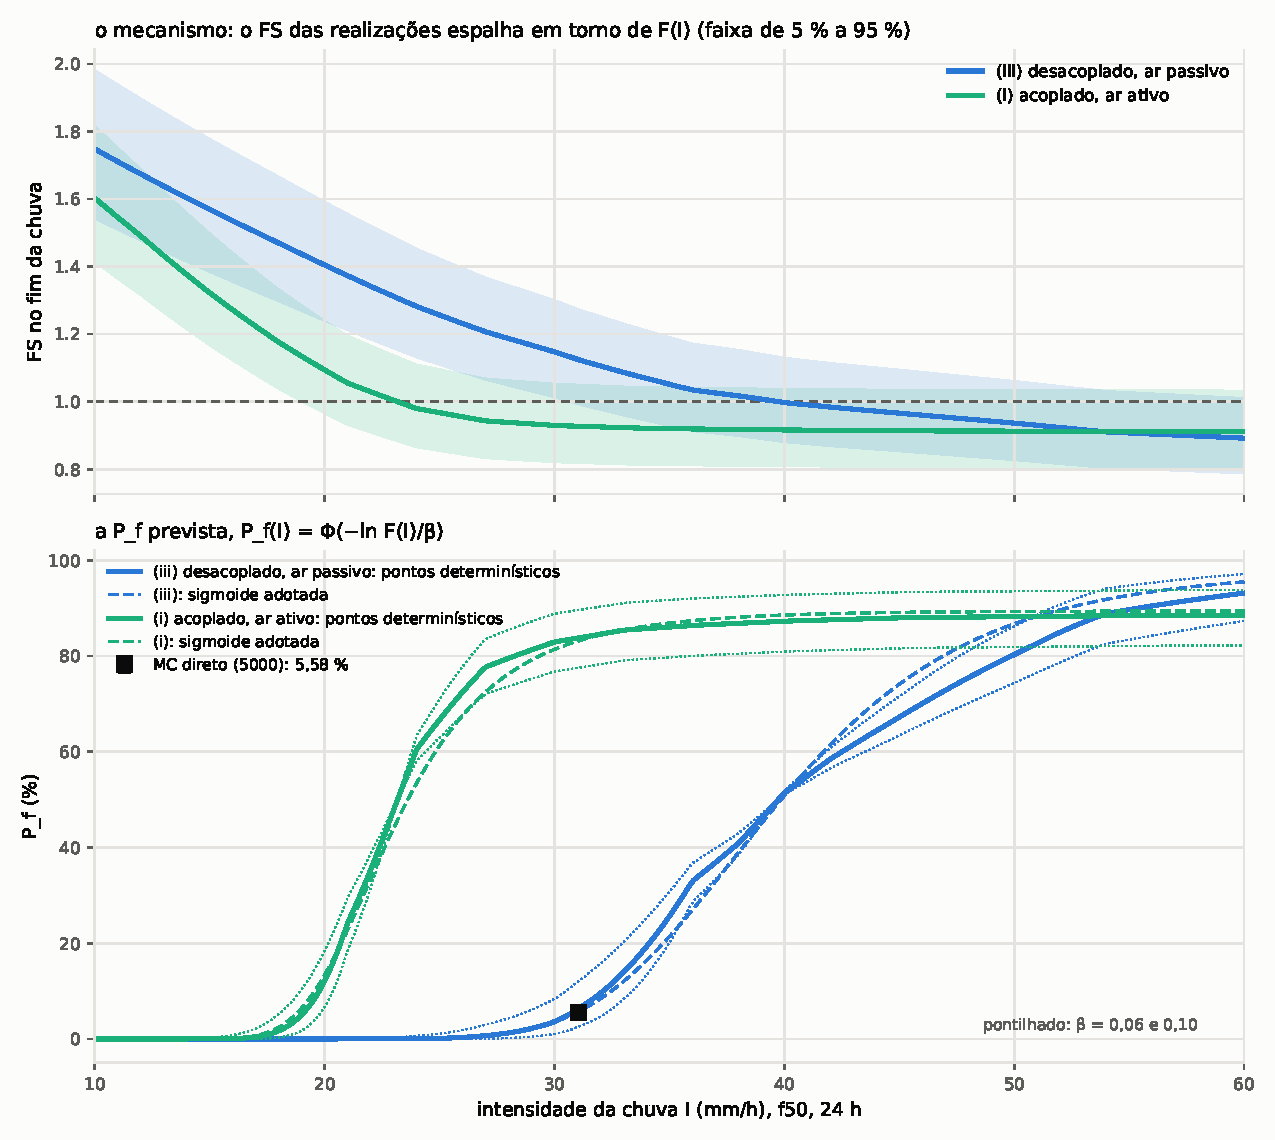
\includegraphics[width=0.85\textwidth]{figs/fragilidade_prevista_f50.pdf}
\caption{f50, chuva de 24~h. Acima: a sigmoide determinística (os pontos interpolados) e a faixa de 5 a 95\,\% do FS
das realizações, $F e^{\pm 1{,}645\beta}$. Abaixo: a $\Pf$ prevista (\ref{eq:frag}) com $\beta = \betaRef$ e $m = 1$
(cheia: os pontos; tracejada: a sigmoide adotada; pontilhada: $\beta$ = 0,06 e 0,10) e o MC direto da referência.}
\label{fig:fragf50}
\end{figure}

\begin{table}[H]\centering\small
\caption{As previsões da campanha \texttt{frag} (f50, 24~h, $m = 1$): $F$ nos pontos determinísticos e a $\Pf$ (\%) com
$\beta = \betaRef$ (pontos e sigmoide adotada) e com $\beta$ = 0,06 e 0,10.}\label{tab:prev}
\begin{tabular}{lccccccc}
\toprule
var. & $I$ (mm/h) & $F$ & $\Pf$, pontos & $\Pf$, sigmoide & $\beta = 0{,}06$ & $\beta = 0{,}10$\\
\midrule
\tabin{tab/previsoes.tex}
\bottomrule
\end{tabular}
\end{table}

\begin{figure}[H]\centering
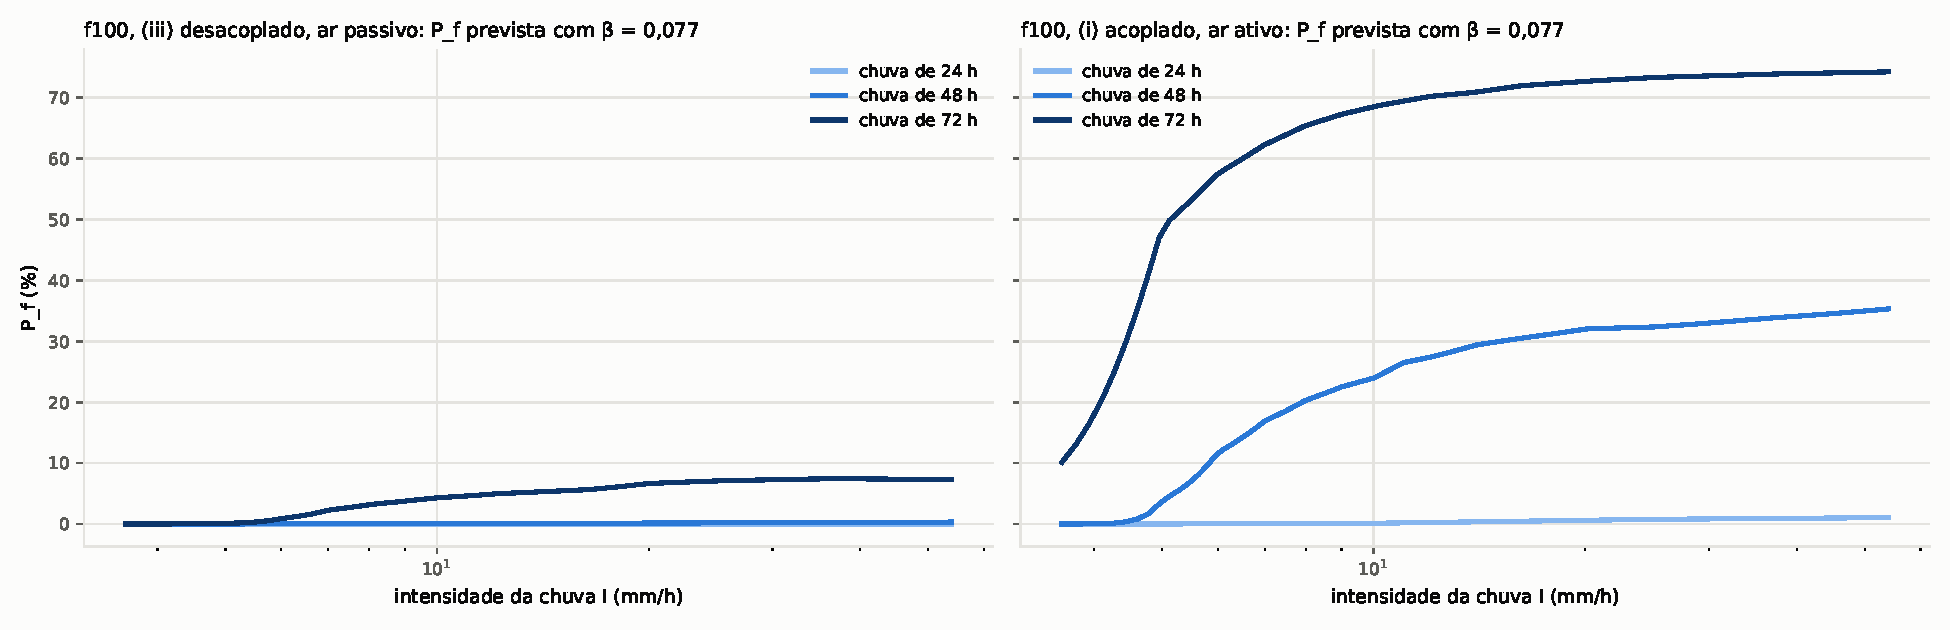
\includegraphics[width=\textwidth]{figs/fragilidade_prevista_f100.pdf}
\caption{f100: a $\Pf$ prevista (\ref{eq:frag}) para chuvas de 24, 48 e 72~h (o FS das médias em cada duração,
$\beta = \betaRef$).}\label{fig:fragf100}
\end{figure}

\begin{itemize}
  \item \textbf{A largura da rampa} no f50: $\sigma_I \approx \sigmaIiii$~mm/h com ar passivo e $\sigmaIi$~mm/h com ar
    ativo. A sigmoide da (i) é mais íngreme em $I_c$ (\declivei{} contra \decliveiii{} em $\ln$ FS por mm/h): com ar
    ativo a passagem de ``quase nunca'' a ``quase sempre'' rompe é mais brusca.
  \item \textbf{A quina em $k_s$ aparece na fragilidade} (iii): a $\Pf$ sobe depressa até 36~mm/h e devagar depois.
    Entre os pontos e a sigmoide suave a diferença chega a 6 pontos (36~mm/h): a forma da sigmoide perto de FS = 1 pesa
    tanto quanto $\beta$.
  \item \textbf{Os patamares limitam a $\Pf$:} com ar ativo ela satura em $\approx 88\,\%$ (o FS das médias não desce de
    0,91); no f100 com 72~h, em $\approx \pfMaxCemiii\,\%$ com ar passivo e $\approx \pfMaxCemi\,\%$ com ar ativo. No
    f100 é a duração, e não a intensidade, que leva à ruptura (Fig.~\ref{fig:fragf100}): acima de $\approx 3k_s$ a
    intensidade quase não importa.
\end{itemize}

\section{A campanha de verificação (\texttt{frag}, fermi)}\label{sec:campanha}
\begin{table}[H]\centering\small
\caption{A campanha \texttt{frag} (\texttt{cluster/casos\_frag.txt}): as mesmas realizações (os campos da referência) em
todos os casos; o f100 só começa depois do f50.}\label{tab:camp}
\begin{tabular}{llp{6.8cm}cc}
\toprule
caso & chuva & intensidades (mm/h) & $N$ & papel\\
\midrule
f50, (iii) & 24~h & $T_1$ em 45, 40, 36, 33, 31,05, 30, 27 & 2000 & verificação\\
f50, (i) & 24~h & $T_1$ em 36, 24, 22, 20, 18 & 2000 & verificação\\
f50, (i) & 24~h & FS em 24~h a 20 & 2000 & $\beta$ e $m$ da (i)\\
f100, (iii) & até 120~h & $T_1$ em 20, 9, 6, 4 & 1000 & verificação\\
f100, (i) & até 120~h & $T_1$ em 20, 9, 5, 3,6 & 1000 & verificação\\
f100, (iii) e (i) & 120~h & FS em 72 e 120~h a 9 e a 3,6 & 1000 & $\beta$ e $m$\\
\bottomrule
\end{tabular}
\end{table}

\begin{itemize}
  \item \textbf{Calibração e previsão separadas:} $\beta$ (e $m$) vêm de uma intensidade só por variante (a referência
    de 5000 na (iii) do f50; os MC de calibração nos outros); as outras intensidades são previsão.
  \item \textbf{Critério:} a fórmula passa se $|z| \le 2$ em todas as intensidades verificadas, com $z = (\Pf^{MC} -
    \Pf^{prev})/\mathrm{EP}$. Com $N = 2000$ o erro padrão da $\Pf$ é de no máximo 1,1 ponto: dá para ver $\beta$
    mudando 20\,\% e o erro da sigmoide na quina.
  \item \textbf{Diagnóstico, se falhar:} (a) H1 --- a lognormal com a mediana e o $\beta$ da própria intensidade
    reproduz a $\Pf$? (b) H2 --- a mediana segue $mF(I)$? (c) $\beta$ é constante? A primeira passagem dá a $\Pf$ de
    cada intensidade exata; os MC de calibração dão a distribuição completa do FS onde for preciso.
  \item \textbf{Conferências embutidas:} a $\Pf$ da primeira passagem tem de reproduzir os MC nas mesmas realizações (a
    31,05~mm/h contra a referência, a 20~mm/h contra a calibração da (i), no f100 a 9 e 3,6~mm/h).
  \item \textbf{Custo:} $\approx 21$~h de fermi (4 nós) para o f50 e $\approx 25$~h para o f100; resultado parcial do
    f50 depois de uma noite. Análise: \path{cluster/resumo_frag.py} (via \path{cluster/baixar_frag.sh}).
\end{itemize}

\section{Simulação de Monte Carlo}\label{sec:mc}
% macros que so existem com dados (o gera_dados.py/mc_secao.py as escreve no numeros.tex)
\providecommand{\mcFormBetaA}{--}\providecommand{\mcFormPfA}{--}\providecommand{\mcFormBetaB}{--}
\providecommand{\mcFormPfB}{--}\providecommand{\mcFragPfA}{--}\providecommand{\mcFragPfB}{--}
\providecommand{\fragZkiii}{--}\providecommand{\fragZkDentroiii}{--}\providecommand{\fragZmiii}{--}
\providecommand{\fragPariii}{--}\providecommand{\fragBetaiii}{--}\providecommand{\fragMkiii}{--}
\providecommand{\fragIcaliii}{--}\providecommand{\fragTopIiii}{--}\providecommand{\fragCensMediii}{--}
\providecommand{\fragCensMedSeiii}{--}\providecommand{\fragCensBetaiii}{--}\providecommand{\fragCensBetaSeiii}{--}
\providecommand{\fragPrevMediii}{--}\providecommand{\fragZki}{--}\providecommand{\fragZkDentroi}{--}
\providecommand{\fragZmi}{--}\providecommand{\fragPari}{--}\providecommand{\fragBetai}{--}\providecommand{\fragMki}{--}
\providecommand{\fragIcali}{--}\providecommand{\fragTemi}{0}\providecommand{\fragTemiii}{0}
\providecommand{\fragZmMaxi}{--}\providecommand{\fragZmDentroi}{--}\providecommand{\fragTopIi}{--}
\providecommand{\fragCensMedi}{--}\providecommand{\fragCensMedSei}{--}\providecommand{\fragCensBetai}{--}
\providecommand{\fragCensBetaSei}{--}\providecommand{\fragPrevMedi}{--}\providecommand{\fragPrevMedMedioi}{--}
\providecommand{\fragCemTem}{0}

Os números desta seção são de \mcData{} e mudam enquanto as rodadas andam: o \texttt{gera.sh} refaz as figuras e as
tabelas com os dados do momento. Em todos os casos o alvo é CoV$(\Pf) = 5\,\%$. As estimativas correntes usam as
realizações (ou as linhas) na ordem do índice, e só o prefixo contínuo das já prontas: as que terminam primeiro são as
mais baratas, e usá-las enviesaria a $\Pf$.

\subsection{Os casos do PC: f50, chuva de 24~h a 30 e 36~mm/h}\label{sec:mcpc}
\begin{itemize}
  \item \textbf{MC direto pela primeira passagem} (a variante (i), com $\Pf$ alta). Cada realização avança de hora em
    hora e confere o FS em 12 e 24~h; se ele cair abaixo de 1, acha $t_1$ por bissecção nas horas guardadas e para ali.
    A fila para o caso no primeiro $N$ com CoV $\le 5\,\%$, com no mínimo 100 realizações e 30 falhas. As realizações
    são as mesmas da campanha \texttt{frag} (a mesma semente).
  \item \textbf{Line sampling} (a variante (iii)). A direção é a do FORM modal, que só tem $c'$ e $\phi'$: o gradiente
    modal dá zero nos termos de $k$, que ficam aleatórios de uma linha para outra. Em cada linha, a raiz de
    FS(24~h)~$= 1$ sai por busca com cerca, com o transiente calculado uma vez por linha. Para na primeira linha com
    CoV $\le 5\,\%$ (no mínimo 30 linhas). O LS não dá $t_1$: o histograma dessas linhas vem do MC do fermi na mesma
    intensidade.
  \item A (iii) a 36~mm/h começou como MC no PC e passou para o LS; o MC dessas realizações segue no fermi.
\end{itemize}

\begin{table}[H]\centering\small
\caption{Os casos do PC (\texttt{\textasciitilde/projects/runs/pc\_f50\_ls\_mc}) e, nas linhas sem rótulo, o MC das mesmas condições.
Fórmula: $\Phi(-\ln(m'F)/\beta)$, com o $F$ do $k_s$ mediano e o $m'$ e o $\beta$ da calibração da variante. CoV do MC:
$\sqrt{(1-\Pf)/(N\Pf)}$; do LS: o desvio padrão das $p_i$ das linhas dividido por $\sqrt N\,\Pf$. ``min/$N$'':
minutos de CPU por realização ou por linha. $t_1$: a mediana e, entre colchetes, os quantis de 10 e 90\,\% das
falhas. O FORM está no texto.}\label{tab:mcpc}
\resizebox{\textwidth}{!}{\begin{tabular}{llrrrrlllrl}
\toprule
caso & método & $N$ & falhas & $\Pf$ (\%) & CoV (\%) & IC 95\,\% & $t_1$ (h) & min/$N$ & fórmula (\%) & estado\\
\midrule
(iii) 30~mm/h & LS & 707 & -- & 3{,}8 & 5{,}0 & 3{,}4--4{,}1 & -- & 4{,}2 & 3{,}8 & CoV 5\,\%\\
 & MC (fermi) & 2000 & 70 & 3{,}5 & 11{,}7 & 2{,}8--4{,}4 & 22{,}6 [20{,}6, 23{,}7] & -- & 3{,}8 & parcial\\
(iii) 36~mm/h & LS & 248 & -- & 23{,}3 & 5{,}0 & 21{,}0--25{,}6 & -- & 6{,}6 & 18{,}0 & CoV 5\,\%\\
 & MC (fermi) & 2000 & 468 & 23{,}4 & 4{,}0 & 21{,}6--25{,}3 & 22{,}2 [19{,}4, 23{,}7] & -- & 18{,}0 & parcial\\
 & MC (PC) & 31 & 4 & 12{,}9 & 46{,}7 & 5{,}1--28{,}9 & 23{,}3 [22{,}0, 23{,}9] & 3{,}0 & 18{,}0 & parado\\
(i) 30~mm/h & MC (PC) & 150 & 129 & 86{,}0 & 3{,}3 & 79{,}5--90{,}7 & 18{,}2 [13{,}7, 21{,}8] & 7{,}9 & 69{,}2 & CoV 5\,\%\\
(i) 36~mm/h & MC (PC) & 120 & 105 & 87{,}5 & 3{,}5 & 80{,}4--92{,}3 & 15{,}8 [10{,}9, 19{,}9] & 7{,}9 & 73{,}6 & CoV 5\,\%\\
\bottomrule
\end{tabular}
}
\end{table}

\begin{figure}[H]\centering
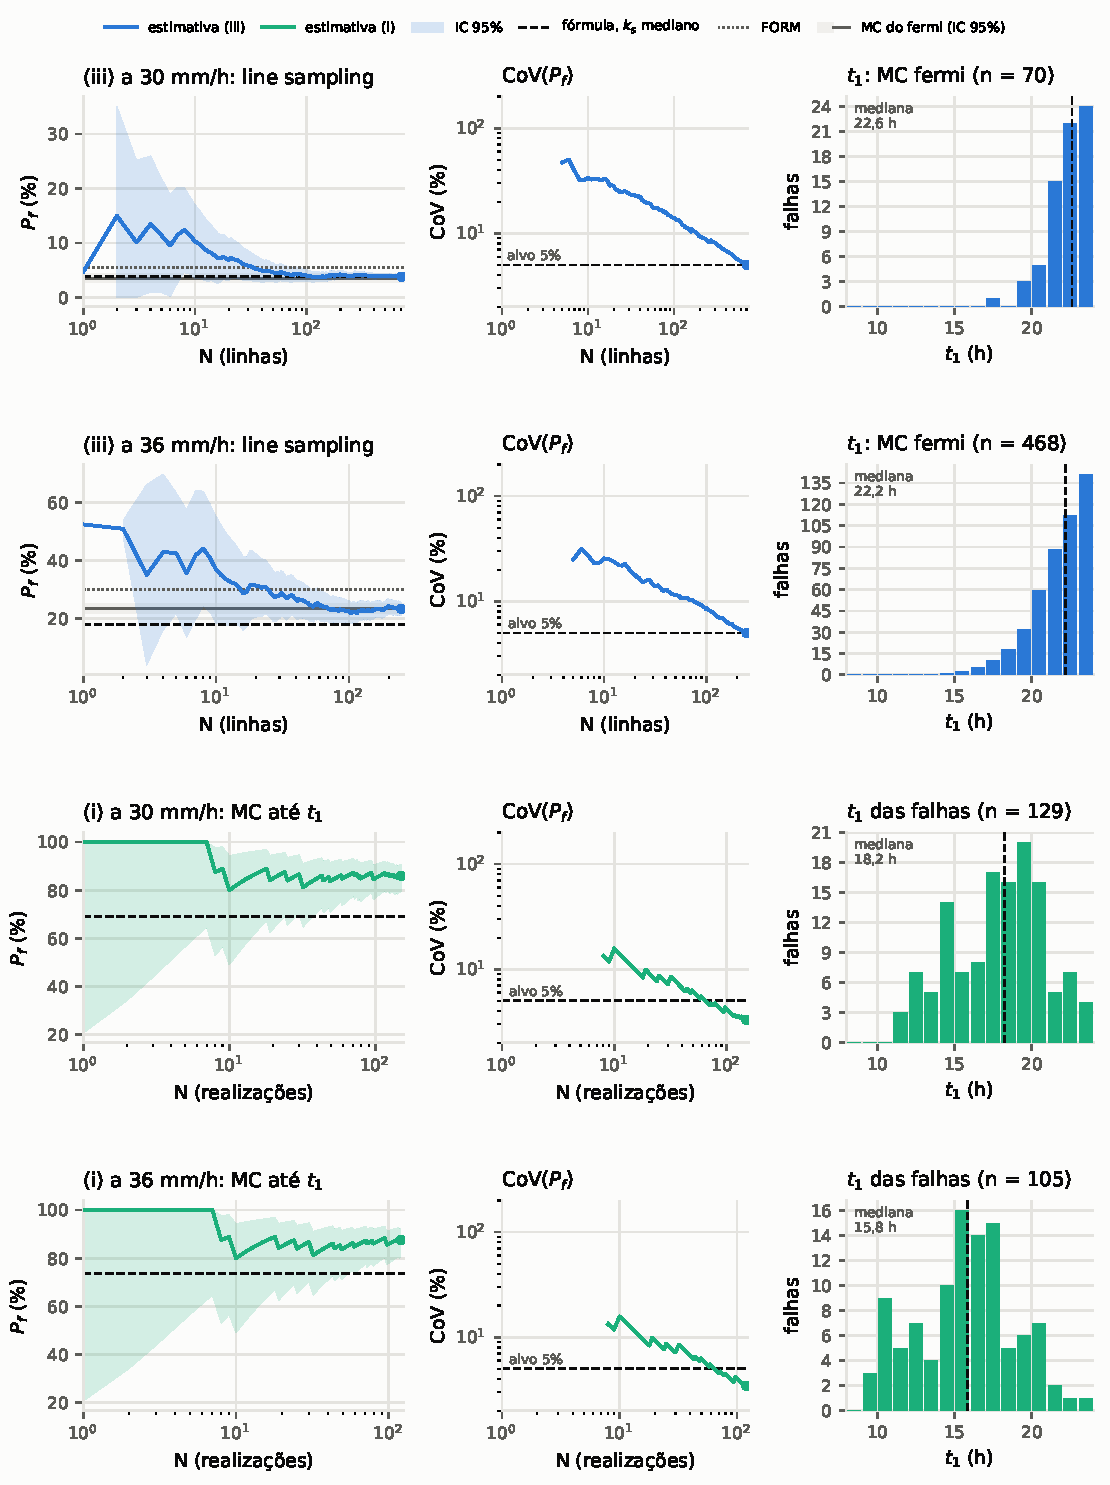
\includegraphics[width=\textwidth]{figs/mc_pc.pdf}
\caption{Os casos do PC, um por linha. Esquerda: a $\Pf$ corrente com o IC de 95\,\% (faixa colorida), a fórmula com o
$k_s$ mediano (tracejada), o FORM (pontilhada) e, no LS, o MC do fermi nas mesmas condições (faixa cinza). Centro: o
CoV$(\Pf)$ e o alvo de 5\,\%. Direita: o histograma de $t_1$ das falhas, com a mediana.}\label{fig:mcpc}
\end{figure}

\begin{itemize}
  \item \textbf{Conferência PC $\times$ fermi} nas mesmas realizações (falhas diferentes): \mcConf. A primeira passagem
    conferida só em 12 e 24~h dá o mesmo $t_1$ que conferida em 6, 12 e 24~h, e a monotonia em $I$ que a campanha usa
    para pular intensidades vale nessas realizações.
  \item \textbf{O FORM perto da mediana.} A 36~mm/h o FORM dá $\Pf = \mcFormPfB\,\%$ ($\beta = \mcFormBetaB$), contra
    $\mcFragPfB\,\%$ do MC do fermi. Com a $\Pf$ perto de 50\,\%, linearizar em $c'$ e $\phi'$ com o $k$ fixo no
    mediano erra muito. O LS não tem viés em nenhuma direção e corrige. A 30~mm/h o FORM ($\mcFormPfA\,\%$,
    $\beta = \mcFormBetaA$) já fica perto do MC ($\mcFragPfA\,\%$).
\end{itemize}

\subsection{A campanha \texttt{frag} no fermi}\label{sec:mcfrag}
O prefixo contínuo de blocos prontos tem \fragNiii{} realizações na (iii) e \fragNi{} na (i). A
Tab.~\ref{tab:fragiii} compara a $\Pf$ de cada intensidade com a fórmula calibrada só a \fragIcaliii~mm/h
($\beta = \fragBetaiii$, $m' = \fragMkiii$). Ela usa o $F$ do $k_s$ médio (a proposta original) e o do $k_s$ mediano.

\ifnum\fragTemiii>0
\begin{table}[H]\centering\small
\caption{A (iii) no \texttt{frag} (primeira passagem, chuva de 24~h). $z = (\Pf^{MC} - \Pf^{prev})/\sqrt{\Pf^{prev}(1 -
\Pf^{prev})/N}$. $F$ médio e $F$ mediano: o FS das médias com o $k_s$ médio e com o mediano; prev.: a fórmula com cada um, em \%.
Pareado: as realizações em que a falha prevista por $\mathrm{FS}_k(I_{cal})\,F(I)/F(I_{cal})$ ($F$ mediano) difere da
observada. $t_1$: a mediana e os quantis de 10 e 90\,\% das falhas.}\label{tab:fragiii}
\resizebox{\textwidth}{!}{\begin{tabular}{rrrrrlrllrl}
\toprule
$I$ & $F$ médio & $F$ mediano & falhas/$N$ & $\Pf$ (\%) & IC 95\,\% & CoV (\%) & prev. médio ($z$) & prev. mediano ($z$) & pareado & $t_1$ (h)\\
\midrule
45 & 0{,}966 & 1{,}012 & 1025/2000 & 51{,}2 & 49{,}1--53{,}4 & 2 & 65{,}7 (-13{,}6) & 38{,}0 (12{,}2) & 473 & 20{,}7 [17{,}0, 23{,}2]\\
40 & 0{,}997 & 1{,}031 & 764/2000 & 38{,}2 & 36{,}1--40{,}4 & 3 & 49{,}7 (-10{,}3) & 29{,}4 (8{,}6) & 323 & 21{,}5 [18{,}3, 23{,}6]\\
36 & 1{,}034 & 1{,}061 & 468/2000 & 23{,}4 & 21{,}6--25{,}3 & 4 & 31{,}4 (-7{,}7) & 18{,}0 (6{,}3) & 177 & 22{,}2 [19{,}4, 23{,}7]\\
33 & 1{,}087 & 1{,}083 & 229/2000 & 11{,}5 & 10{,}1--12{,}9 & 6 & 13{,}0 (-2{,}1) & 11{,}9 (-0{,}6) & 52 & 22{,}6 [19{,}9, 23{,}8]\\
31{,}05 & 1{,}124 & 1{,}115 & 109/2000 & 5{,}5 & 4{,}5--6{,}5 & 9 & 5{,}9 (-0{,}8) & 5{,}9 (-0{,}8) & 0 & 22{,}6 [20{,}4, 23{,}8]\\
30 & 1{,}148 & 1{,}133 & 70/2000 & 3{,}5 & 2{,}8--4{,}4 & 12 & 3{,}3 (0{,}5) & 3{,}8 (-0{,}8) & 5 & 22{,}6 [20{,}6, 23{,}7]\\
27 & 1{,}207 & 1{,}195 & 13/2000 & 0{,}7 & 0{,}4--1{,}1 & 28 & 0{,}6 (0{,}1) & 0{,}7 (-0{,}2) & 9 & 23{,}4 [22{,}0, 23{,}6]\\
\bottomrule
\end{tabular}
}
\end{table}

\begin{figure}[H]\centering
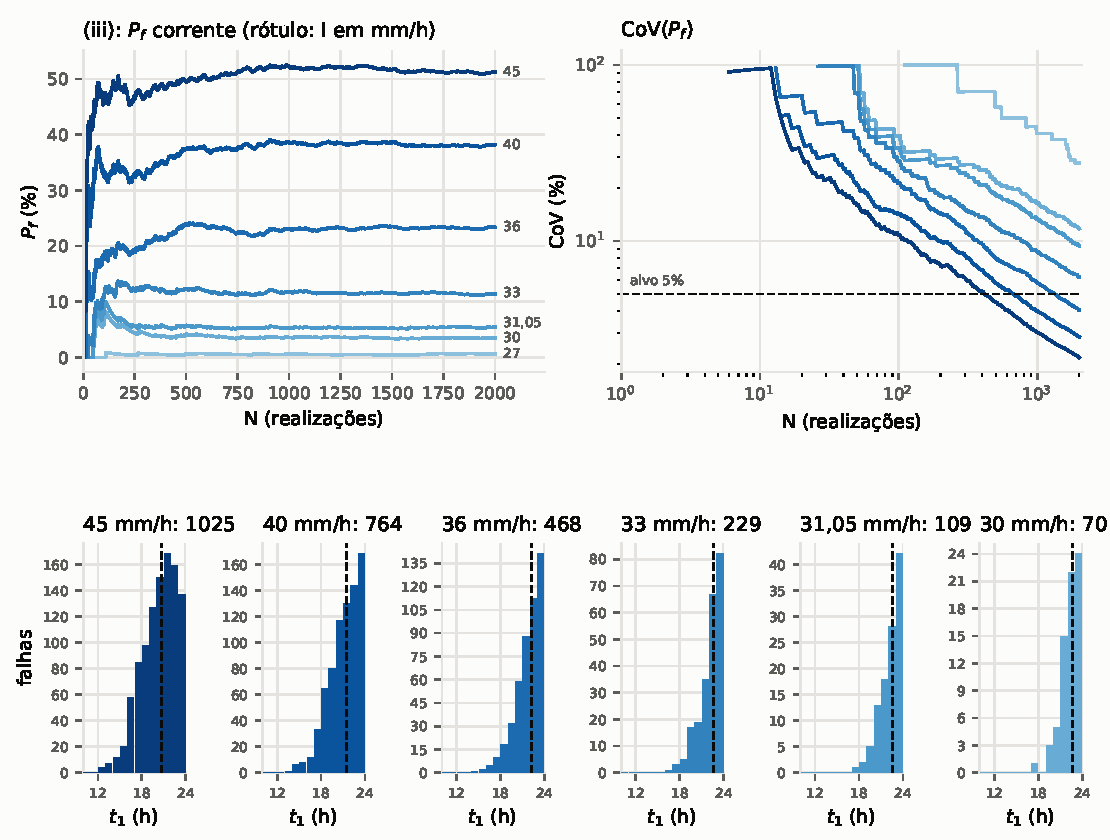
\includegraphics[width=\textwidth]{figs/frag_iii.pdf}
\caption{A (iii) no \texttt{frag}. Acima: a $\Pf$ corrente e o CoV de cada intensidade (rótulo: $I$ em mm/h; cor mais
escura, $I$ maior). Abaixo: o histograma de $t_1$ nas intensidades com falhas (título: $I$ e o número de falhas), com a
mediana.}\label{fig:fragiii}
\end{figure}

\begin{itemize}
  \item \textbf{Até $\approx k_s$ a fórmula acerta; acima dele, não.} Com o $F$ do $k_s$ médio, a fórmula superestima a $\Pf$ acima de $k_s$
    ($z$ chega a \fragZmiii). Com o $F$ do $k_s$ mediano, $|z| \le \fragZkiii$, e \fragZkDentroiii{} intensidades ficam
    com $|z| \le 2$. O $k_s$ mediano é a média geométrica, a condutividade efetiva de um campo lognormal em 2D. Nada foi
    ajustado aos dados do \texttt{frag}: $m'$ e $\beta$ vêm da calibração.
  \item \textbf{A fórmula vale para a distribuição, não para cada realização.} O teste pareado prevê a falha de cada
    realização por $\mathrm{FS}_k(I) = \mathrm{FS}_k(I_{cal})\,F(I)/F(I_{cal})$ e conta as divergências com a primeira
    passagem ($I$: divergências): \fragPariii. Acima do $k_s$ as realizações trocam de ordem: as de $k$ alto passam a
    ser as mais fracas.
  \item \textbf{$\beta$ na maior intensidade.} A \fragTopIiii~mm/h todas as realizações rodam. Com o FS de 24~h das
    sobreviventes e só a contagem das falhas, a lognormal censurada dá mediana \fragCensMediii~$\pm$~\fragCensMedSeiii{}
    (prevista \fragPrevMediii) e $\beta = \fragCensBetaiii \pm \fragCensBetaSeiii$ (calibrado \fragBetaiii).
\end{itemize}
\fi

\ifnum\fragTemi>0
\begin{table}[H]\centering\small
\caption{A (i) no \texttt{frag}, como na Tab.~\ref{tab:fragiii}; calibração a \fragIcali~mm/h ($\beta = \fragBetai$,
$m' = \fragMki$).}\label{tab:fragi}
\resizebox{\textwidth}{!}{\begin{tabular}{rrrrrlrllrl}
\toprule
$I$ & $F$ médio & $F$ mediano & falhas/$N$ & $\Pf$ (\%) & IC 95\,\% & CoV (\%) & prev. médio ($z$) & prev. mediano ($z$) & pareado & $t_1$ (h)\\
\midrule
36 & 0{,}919 & 0{,}929 & 1651/2000 & 82{,}5 & 80{,}8--84{,}2 & 1 & 87{,}8 (-7{,}1) & 73{,}6 (9{,}1) & 398 & 14{,}8 [11{,}5, 20{,}0]\\
24 & 0{,}980 & 0{,}972 & 1133/2000 & 56{,}6 & 54{,}5--58{,}8 & 2 & 66{,}1 (-8{,}9) & 54{,}1 (2{,}3) & 295 & 20{,}4 [17{,}0, 23{,}2]\\
22 & 1{,}029 & 1{,}003 & 778/2000 & 38{,}9 & 36{,}8--41{,}1 & 3 & 43{,}5 (-4{,}2) & 39{,}6 (-0{,}6) & 139 & 21{,}5 [18{,}2, 23{,}5]\\
20 & 1{,}094 & 1{,}057 & 353/2000 & 17{,}6 & 16{,}0--19{,}4 & 5 & 19{,}0 (-1{,}5) & 19{,}0 (-1{,}5) & 0 & 22{,}0 [19{,}5, 23{,}7]\\
18 & 1{,}176 & 1{,}139 & 114/2000 & 5{,}7 & 4{,}8--6{,}8 & 9 & 4{,}2 (3{,}3) & 3{,}9 (4{,}0) & 43 & 22{,}9 [21{,}3, 23{,}8]\\
\bottomrule
\end{tabular}
}
\end{table}

\begin{figure}[H]\centering
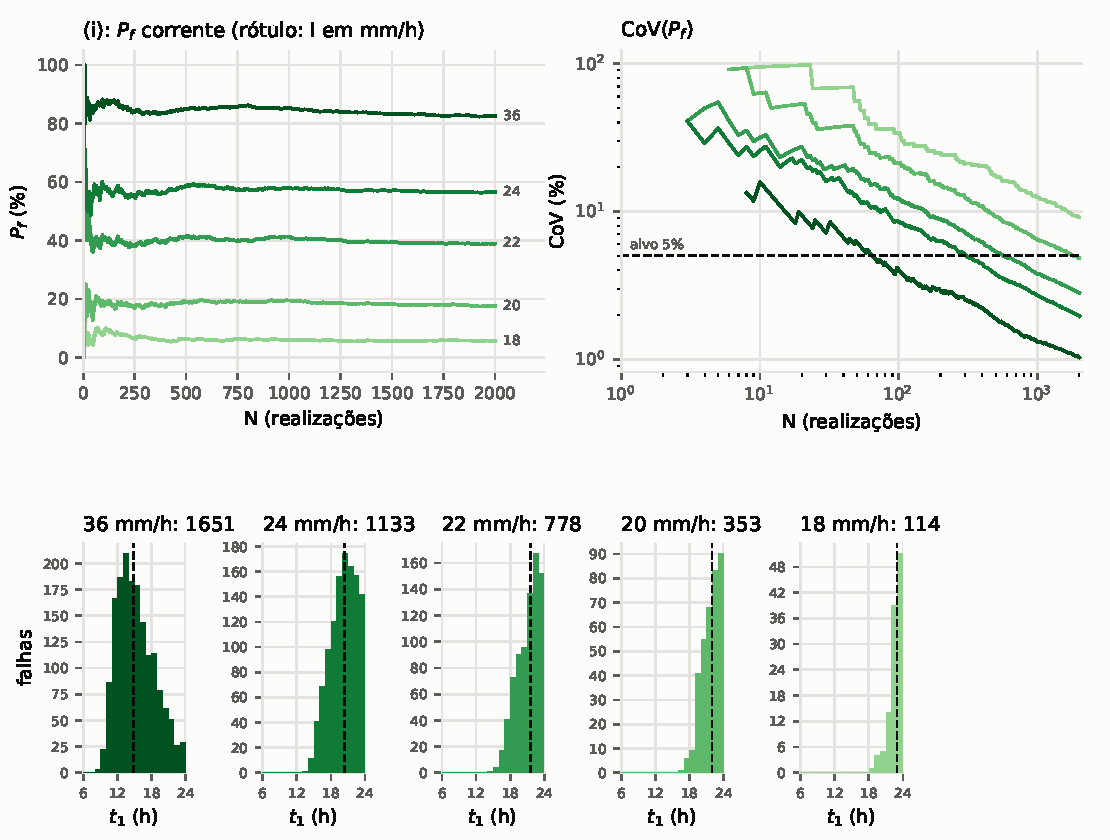
\includegraphics[width=\textwidth]{figs/frag_i.pdf}
\caption{A (i) no \texttt{frag}, como na Fig.~\ref{fig:fragiii}.}\label{fig:fragi}
\end{figure}

\begin{itemize}
  \item \textbf{Na (i), quase o mesmo quadro.} Com o $F$ do $k_s$ mediano,
    \fragZkDentroi{} intensidades ficam com $|z| \le 2$ ($|z|$ chega a \fragZki); com o do $k_s$ médio,
    \fragZmDentroi{} ($|z|$ até \fragZmMaxi). A diferença para a (iii) é a menor intensidade, 18~mm/h, abaixo da
    calibração e do $k_s$: a fórmula dá 3,9\,\% contra 5,7\,\% do MC ($z = 4$). Com ar ativo a cauda abaixo da
    calibração também foge, e a fórmula ali fica contra a segurança.
  \item \textbf{O FS cai mais que $F$ e espalha mais na maior intensidade.} A \fragTopIi~mm/h, a lognormal censurada dá
    mediana \fragCensMedi~$\pm$~\fragCensMedSei{} (prevista \fragPrevMedMedioi{} com o $k_s$ médio e \fragPrevMedi{}
    com o mediano) e $\beta = \fragCensBetai \pm \fragCensBetaSei$ (calibrado \fragBetai).
  \item \textbf{Realização por realização,} como na (iii), a escala só vale perto da intensidade da calibração
    ($I$: divergências): \fragPari.
  \item \textbf{A ruptura vem mais cedo com ar ativo:} a mediana de $t_1$ a 36~mm/h é de $\approx 16$~h na (i),
    contra $\approx 22$~h na (iii) (Tabs.~\ref{tab:fragiii} e \ref{tab:fragi}).
  \item \textbf{Nas duas variantes, o que foge da fórmula é a maior intensidade, e é o $\beta$ que cresce ali}
    (\fragBetaiii{} $\to$ \fragCensBetaiii{} na (iii) a \fragTopIiii~mm/h; \fragBetai{} $\to$ \fragCensBetai{} na (i)
    a \fragTopIi~mm/h). É o $\beta(I)$ acima do $k_s$ que a Seção~\ref{sec:riscos} antecipava: a fórmula com um
    $\beta$ só vale até $\approx k_s$, e acima dele pede um segundo $\beta$.
\end{itemize}
\else
A (i) ainda não tem bloco pronto no prefixo: o primeiro bloco, com a determinística, ainda roda.
\fi

\ifnum\fragCemTem>0
\subsection{O f100 no \texttt{frag} (parcial): a duração}\label{sec:mcf100}
A chuva vai até 120~h, mas a falha que entra na comparação é a de até 72~h, a duração das sigmoides do f100. A fórmula
usa o $F$ das médias com o $k_s$ médio (o f100 ainda não tem a sigmoide do $k_s$ mediano), e o $\beta$ e o $m$ vêm do
MC de calibração, com o FS em 72~h: (iii) a \fragCemIcaliii~mm/h ($\beta = \fragCemBetaiii$, $m = \fragCemMiii$,
\fragCemNcaliii{} realizações) e (i) a \fragCemIcali~mm/h ($\beta = \fragCemBetai$, $m = \fragCemMi$, \fragCemNcali).

\begin{table}[H]\centering\small
\caption{O f100 no \texttt{frag}: o prefixo contínuo de \fragCemNiii{} realizações na (iii) e \fragCemNi{} na (i), de
1000. $F$: o FS das médias em 72~h. $\Pf$: a falha até 72~h, com o IC de 95\,\%; prev.: a fórmula com o $\beta$ e o $m$
da calibração, e $z$ como na Tab.~\ref{tab:fragiii}. 48, 60 e 96~h: a $\Pf$ (\%) para essas durações, pela mesma
primeira passagem. $t_1$: a mediana e os quantis de 10 e 90\,\% das falhas até 72~h.}\label{tab:fragf100}
\resizebox{\textwidth}{!}{\begin{tabular}{llrrrlllll l}
\toprule
variante & $I$ & $F$ (72 h) & falhas/$N$ & $\Pf$ (\%) & IC 95\,\% & prev. ($z$) & 48 h & 60 h & 96 h & $t_1$ (h)\\
\midrule
(iii) & 20 & 1{,}122 & 59/466 & 12{,}7 & 9{,}9--16{,}0 & 10{,}2 (1{,}8) & 0{,}9 & 4{,}3 & 39{,}1 & 62{,}5 [48{,}7, 69{,}7]\\
(iii) & 9 & 1{,}146 & 32/466 & 6{,}9 & 4{,}9--9{,}5 & 6{,}9 (0{,}0) & 0{,}0 & 1{,}9 & 31{,}5 & 66{,}5 [56{,}4, 71{,}1]\\
(iii) & 6 & 1{,}199 & 3/466 & 0{,}6 & 0{,}2--1{,}9 & 2{,}6 (-2{,}6) & 0{,}0 & 0{,}0 & 14{,}8 & 66{,}8 [65{,}8, 70{,}2]\\
(iii) & 4 & 1{,}419 & 0/466 & 0{,}0 & 0{,}0--0{,}8 & 0{,}0 (-0{,}2) & 0{,}0 & 0{,}0 & 0{,}0 & --\\
\midrule
(i) & 20 & 0{,}955 & 306/468 & 65{,}4 & 61{,}0--69{,}6 & 70{,}5 (-2{,}4) & 31{,}8 & 49{,}1 & 84{,}8 & 48{,}5 [30{,}7, 67{,}3]\\
(i) & 9 & 0{,}966 & 278/468 & 59{,}4 & 54{,}9--63{,}8 & 65{,}1 (-2{,}6) & 24{,}8 & 43{,}2 & 82{,}1 & 51{,}2 [35{,}8, 67{,}3]\\
(i) & 5 & 1{,}002 & 200/468 & 42{,}7 & 38{,}3--47{,}3 & 47{,}0 (-1{,}9) & 2{,}4 & 23{,}1 & 74{,}4 & 59{,}6 [50{,}2, 69{,}1]\\
(i) & 3{,}6 & 1{,}103 & 43/468 & 9{,}2 & 6{,}9--12{,}1 & 10{,}1 (-0{,}6) & 0{,}0 & 0{,}4 & 52{,}4 & 67{,}5 [63{,}6, 70{,}8]\\
\bottomrule
\end{tabular}
}
\end{table}

\begin{itemize}
  \item \textbf{A fórmula passa raspando.} Na (iii), 3 das 4 intensidades com $|z| \le 2$; a 6~mm/h ela dá 2,6\,\%
    contra 0,6\,\% (3 falhas em 466, $z = -2{,}6$), do lado conservador. Na (i), as duas maiores intensidades ficam
    com $z \approx -2{,}5$: a fórmula dá $\approx 5$ pontos a mais (70 contra 65\,\% a 20~mm/h), também conservadora.
    Com metade das realizações, o critério $|z| \le 2$ ainda não decide; o resultado completo dirá.
  \item \textbf{No f100 é a duração que manda.} Com ar passivo, a 20 e a 9~mm/h a $\Pf$ vai de $\approx 1\,\%$ em
    48~h para 31--39\,\% em 96~h; a intensidade importa pouco acima de $\approx 3k_s$. Com ar ativo a $\Pf$ em 72~h
    já passa de 40\,\% a 5~mm/h, e o $t_1$ das falhas é mais cedo e mais espalhado (mediana de 49--60~h, contra 62--67~h
    com ar passivo).
  \item \textbf{$\beta$ cresce com a duração.} No MC de calibração, de 72 para 120~h, $\beta$ vai de \fragCemBetaiii{}
    a \fragCemBetaCxxiii{} na (iii) e de \fragCemBetai{} a \fragCemBetaCxxi{} na (i). Para $\Pf(I, D)$ a fórmula
    precisa de $\beta(D)$, ou de uma calibração por duração.
\end{itemize}
\fi

\section{Hipóteses e o que pode falhar}\label{sec:riscos}
\begin{itemize}
  \item \textbf{$\beta$ pode mudar com $I$.} Abaixo de $k_s$ toda a chuva entra e o $k_s$ não pesa (Spearman de $k_s$
    com o FS $\approx 0$ na referência); acima, com alagamento, a variabilidade de $k_s$ entra e $\beta$ deve crescer.
    Se crescer, a fórmula precisa de $\beta(I/k_s)$ (por exemplo, dois valores, abaixo e acima de $k_s$).
  \item \textbf{A forma da sigmoide.} A quina em $k_s$ não é capturada por nenhuma forma suave; uma sigmoide em dois
    trechos, $I < k_s$ e $I > k_s$, ou o uso direto dos pontos determinísticos interpolados, resolvem.
  \item \textbf{A mediana contra o FS das médias} ($m$): constante? A campanha mede $m$ em duas intensidades por
    variante.
  \item \textbf{A cauda lognormal} abaixo de 1\,\%: a referência confirma até $\approx 0{,}5\,\%$; abaixo, só com LS ou
    mais realizações.
  \item \textbf{As monotonias} (o FS só cai durante a chuva; $T_1$ cai com $I$): valem em todos os casos calculados; a
    campanha as confere nas conferências embutidas.
  \item \textbf{A validação determinística} (em pausa; \path{plano_deterministico.md}): a malha do SRM ainda não
    convergiu ($\approx 0{,}01$ no FS), a malha do transiente é grossa e a chuva entra por metro inclinado. Isso muda
    os números absolutos, mas não o teste da fórmula: a sigmoide e o MC vêm do mesmo código, e um erro sistemático
    desloca os dois juntos.
  \item \textbf{A generalidade.} $\beta$ depende das estatísticas dos campos (CoV, distâncias de autocorrelação,
    anisotropia): as famílias da Seção~6 de Vargas Ceron et al.\ (2025) mapeariam $\beta$; $A, B, C, D_s$ dependem do
    talude e do solo (Rahardjo usa $I/k_s$ para comparar solos).
\end{itemize}

\section{Próximos passos}
\begin{enumerate}
  \item \textbf{Feito (f50 completo):} com um $\beta$ só o critério $|z| \le 2$ falha acima de $k_s$ (e, com ar ativo,
    também a 18~mm/h). O diagnóstico aponta para $\beta(I)$: a forma corrigida a testar é $\beta$ em dois trechos
    ($I < k_s$ e $I > k_s$), com a segunda calibração na maior intensidade, e conferir se ela fecha as intensidades
    intermediárias.
  \item O f100 completo (1000 realizações): o critério em 72~h e a $\Pf(I, D)$ com $\beta(D)$; os limiares da
    Eq.~\ref{eq:limiar}.
  \item A sigmoide do $k_s$ mediano no f100, como no f50.
  \item Retomar a validação determinística e refazer os números finais com a malha e a convenção da chuva decididas.
\end{enumerate}


\begin{thebibliography}{99}\small
\bibitem{rahardjo2007} H.~Rahardjo, T.~H.~Ong, R.~B.~Rezaur, E.~C.~Leong. Factors controlling instability of
  homogeneous soil slopes under rainfall. \emph{Journal of Geotechnical and Geoenvironmental Engineering}
  133(12):1532--1543, 2007. \url{https://doi.org/10.1061/(ASCE)1090-0241(2007)133:12(1532)}
\bibitem{ceron2025} M.~Vargas Ceron, D.~L.~Cecílio, R.~V.~Linn, S.~Maghous. Stability analysis of slope subjected to
  seepage forces considering spatial variability of soil properties. \emph{International Journal for Numerical and
  Analytical Methods in Geomechanics}, 2025. \url{https://doi.org/10.1002/nag.3993}
\bibitem{liuwang2023} X.~Liu, Y.~Wang. Probabilistic hazard analysis of rainfall-induced landslides at a specific slope
  considering rainfall uncertainty and soil spatial variability. \emph{Computers and Geotechnics} 162:105706, 2023.
  \url{https://doi.org/10.1016/j.compgeo.2023.105706}
\bibitem{hu2024} H.~Hu, Y.~Bao, X.~Han, W.~Wang. Non-parametric fragility curves for probabilistic risk assessment of
  rainfall-triggered landslides. \emph{Computers and Geotechnics} 173:106546, 2024.
  \url{https://doi.org/10.1016/j.compgeo.2024.106546}
\bibitem{liu2024} L.-L.~Liu, H.~Han, S.-Y.~Huang, L.~Huang, Y.-M.~Cheng. Combined influence of rotated transverse
  anisotropy in mechanical parameters and hydraulic conductivity of soils on reliability evaluation of an unsaturated
  slope under rainfalls. \emph{Computers and Geotechnics} 165:105938, 2024.
  \url{https://doi.org/10.1016/j.compgeo.2023.105938}
\bibitem{cho2014} S.~E.~Cho. Probabilistic stability analysis of rainfall-induced landslides considering spatial
  variability of permeability. \emph{Engineering Geology} 171:11--20, 2014.
  \url{https://doi.org/10.1016/j.enggeo.2013.12.015}
\bibitem{cho2020} S.~E.~Cho. Failure distribution analysis of shallow landslides under rainfall infiltration based on
  fragility curves. \emph{Landslides} 17:79--91, 2020. \url{https://doi.org/10.1007/s10346-019-01257-w}
\bibitem{xliu2025} X.~Liu, S.-H.~Jiang, J.~Xie, X.~Li. Bayesian inverse analysis with field observation for slope
  failure mechanism and reliability assessment under rainfall accounting for nonstationary characteristics of soil
  properties. \emph{Soils and Foundations} 65:101568, 2025. \url{https://doi.org/10.1016/j.sandf.2025.101568}
\bibitem{tang2018} G.~Tang, J.~Huang, D.~Sheng, S.~W.~Sloan. Stability analysis of unsaturated soil slopes under random
  rainfall patterns. \emph{Engineering Geology} 245:322--332, 2018. \url{https://doi.org/10.1016/j.enggeo.2018.09.013}
\bibitem{yang2026} R.~Yang, Y.~Meng, G.~Cai, J.~Huang. A novel framework for reliability analysis of rainfall-induced
  slopes failure based on site-specific data. \emph{International Journal for Numerical and Analytical Methods in
  Geomechanics} 50:5213--5229, 2026. \url{https://doi.org/10.1002/nag.70370}
\bibitem{su2026} C.~Su, A.~Che, H.~Zhou, G.~Yuan, J.~Zhou. Effect of strength spatial variability on the probabilistic
  post-landslide behavior of heterogeneous slopes under rainfall. \emph{International Journal for Numerical and
  Analytical Methods in Geomechanics} 50:4633--4652, 2026. \url{https://doi.org/10.1002/nag.70350}
\bibitem{dou2015} H.-q.~Dou, T.-c.~Han, X.-n.~Gong, Z.-y.~Qiu, Z.-n.~Li. Effects of the spatial variability of
  permeability on rainfall-induced landslides. \emph{Engineering Geology} 192:92--100, 2015.
  \url{https://doi.org/10.1016/j.enggeo.2015.03.014}
\bibitem{qian2025} C.~Qian et al. Temporal stability and risk analysis of soil slopes subject to rainfall: the influence
  of heterogeneity. \emph{Engineering Geology} 347:107895, 2025. \url{https://doi.org/10.1016/j.enggeo.2024.107895}
\bibitem{masoudian2019} M.~S.~Masoudian, M.~A.~Hashemi Afrapoli, A.~Tasalloti, A.~M.~Marshall. A general framework for
  coupled hydro-mechanical modelling of rainfall-induced instability in unsaturated slopes with multivariate random
  fields. \emph{Computers and Geotechnics} 115:103162, 2019. \url{https://doi.org/10.1016/j.compgeo.2019.103162}
\bibitem{pan2024} M.~Pan, S.-H.~Jiang, X.~Liu, G.-Q.~Song, J.~Huang. Sequential probabilistic back analyses of
  spatially varying soil parameters and slope reliability prediction under rainfall. \emph{Engineering Geology}
  328:107372, 2024. \url{https://doi.org/10.1016/j.enggeo.2023.107372}
\bibitem{le2019} T.~M.~H.~Le, M.~Sanchez, D.~Gallipoli, S.~Wheeler. Probabilistic study of rainfall-triggered
  instabilities in randomly heterogeneous unsaturated finite slopes. \emph{Transport in Porous Media} 126:199--222,
  2019. \url{https://doi.org/10.1007/s11242-018-1140-0}
\bibitem{demisa2025} M.~G.~Demisa, S.~Wang, Q.~Hou, S.~Wenpan, F.~Dong, B.~Han. A probabilistic framework for
  rainfall-induced instability in unsaturated slopes using bivariate rainfall and multivariate soil random fields.
  \emph{Bulletin of Engineering Geology and the Environment} 84:207, 2025.
  \url{https://doi.org/10.1007/s10064-025-04171-9}
\end{thebibliography}

\end{document}
